\chapter{Basis Sets}
\label{chap:basis_sets}
\section{Introduction}
As stated in section \ref{subsec:basis_sets}, the use of Gaussian-type functions is the favored way of constructing basis sets for the use in molecular calculations. The use of basis sets introduces a new source of error, as we are now only approximating a wavefunction instead of directly numerically calculating it. One of the ways this error can manifest itself is in basis set superposition error (BSSE). BSSE appears when comparing the differences in energy between two different systems, as one might do to compare the difference in energy between reactants and product in a chemical reaction. 

\notetodylan{For instance, we might want to find the energy of the reaction $\text{H}^{+} + \text{OH}^{-} \rightarrow \text{H}_{2}\text{O}$. The calculation of $\text{H}_{2}\text{O}$ will have three basis functions centers while the $\text{OH}^{-}$ calculation will only have two. The $\text{OH}^{-}$ fragment inside the $\text{H}_{2}\text{O}$ molecule will have additional basis functions from the $\text{H}^{+}$ fragment to work with while the $\text{OH}^{-}$ does not. As a result, the $\text{OH}^{-}$ fragment and molecule are not being described exactly the same, and therefore errors can result from this.}

%Because we can not use a basis set with an infinite amount of basis functions, the basis set for the products and reactants in this example will be different (each will potentially have a different number of basis function centers, locations, etc.). This means that we are not comparing calculations with exactly the same level of accuracy, and the results may be invalidated because of this. 

There is also the possibility of approximate linear dependencies in the basis set, which may show up during the SCF process. This happens when the overlap between any two different functions is close to unity (at least as far as a double precision number is concerned) and will mean that there will be eigenvalues that are equal to zero when diagonalizing the overlap matrix. We cannot find the inverse of such a matrix, so therefore the functions leading to these eigenvalues of zero must get transformed out of the matrix. This is kind of bandaid solution though, as the resulting Fock matrix after this transformation could produce errors in the energy differences on the order of chemical accuracy. It can also lead to a very aggravating process during a geometry optimization. 

For example, say we have a molecular system in geometry state A. In this state, there are no approximate linear dependencies, and the geometry optimizer determines that the system would prefer to be in geometry state B. It updates the geometry, but in state B, some atoms might be too close together and now there are eigenfunctions that need to be rejected. The energy calculated for geometry state B is inaccurate, which causes the geometry optimizer to think that it should place the atoms back into state A. But now, everything is exactly the same as it was, and the geometry optimizer, with no memory at all of what just happened, thinks that the perfect geometry is state B again. There is no way out of this loop, and we will not be able to find a stationary state, and all because of a poor choice in basis set. It is therefore important for a computational chemist to be aware of these issues so they can identify them when they occur, but even more so for someone who wants to make a new basis set, so that these issues can be avoided in the first place.

Designing a basis set that reduces the effects of BSSE is relatively straightforward, we can simply brute force the problem by adding more and more functions until they begin to cancel each other out. Designing one that avoids the issue of approximate linear dependencies however is more tricky. It is simply not possible to test every possible combination of atoms in every possible geometry to determine if a basis set has these problems. But there are some strategies we can use to avoid this problem.

One strategy that has shown to be particularly effective is using an exponent generating function to ensure that the exponents of the basis set are sufficiently different. There are many of these generating functions. One of these give what are called even-tempered basis sets (ETBS)\cite{ETBS}. The generating function for an ETBS is given below

\begin{equation}
\label{eq:ETBS_gen}
\zeta_{l,k} = \alpha_{l}\beta^{k-1}_{l}, \quad \alpha_{l}, \beta_{l} > 0, \quad \beta_{l} \neq 1, \quad k = 1, 2, \ldots
\end{equation}

where $\zeta_{l,k}$ is the $k^{\text{th}}$ exponent of basis function for orbital symmetry $l$, $\alpha_{l}$ is the exponent for the first, most diffuse, basis function, and $\beta_{l}$ is a growth parameter that determines the gap between $\zeta_{l,k}$ and $\zeta_{l,k + 1}$. This greatly reduces the difficulty of the problem, because instead of needing to optimize all the exponents of our basis set, we only need to optimize the $\alpha$ and $\beta$ parameters of each symmetry. We can further reduce the number of parameters to optimize by using the same $\alpha$ and $\beta$ parameters \textit{for each symmetry}. This is what I did for the work in this chapter, so I will drop the $l$ subscript. However, there is a problem with ETBS: the growth in the value of the exponents is not always sufficient. So we get diminishing returns by increasing the maximum value of $k$, and we have to add many more functions to improve the accuracy of the basis set by even a small amount. This is improved in the well-tempered basis set (WTBS)\cite{WTBS} generating function, which is shown below

\begin{equation}
\label{eq:WTBS_gen}
\zeta_{k} = \zeta_{k-1}\beta\left[1+\gamma\left(\frac{k}{n}\right)^{\delta}\right], \quad k = 2, 3,\ldots, n, \quad \zeta_{1}=\alpha
\end{equation}

where $n$ is the maximum number of basis functions for the set, and $\alpha$ and $\beta$ have the same restrictions on them as they did before. The parameters $\delta$ and $\gamma$ have the effect of increasing the gap between $\zeta$s caused by $\beta$ at high $k$. This means that the growth of the exponents is increased as they get larger, which allows them to make a more meaningful contribution to the total wavefunction. Thus, we get a more accurate basis set with far fewer functions. The effect that altering $\gamma$ and $\delta$ has on the exponents can be seen in Figure \ref{fig:deltagamm}.

\begin{figure}
\center
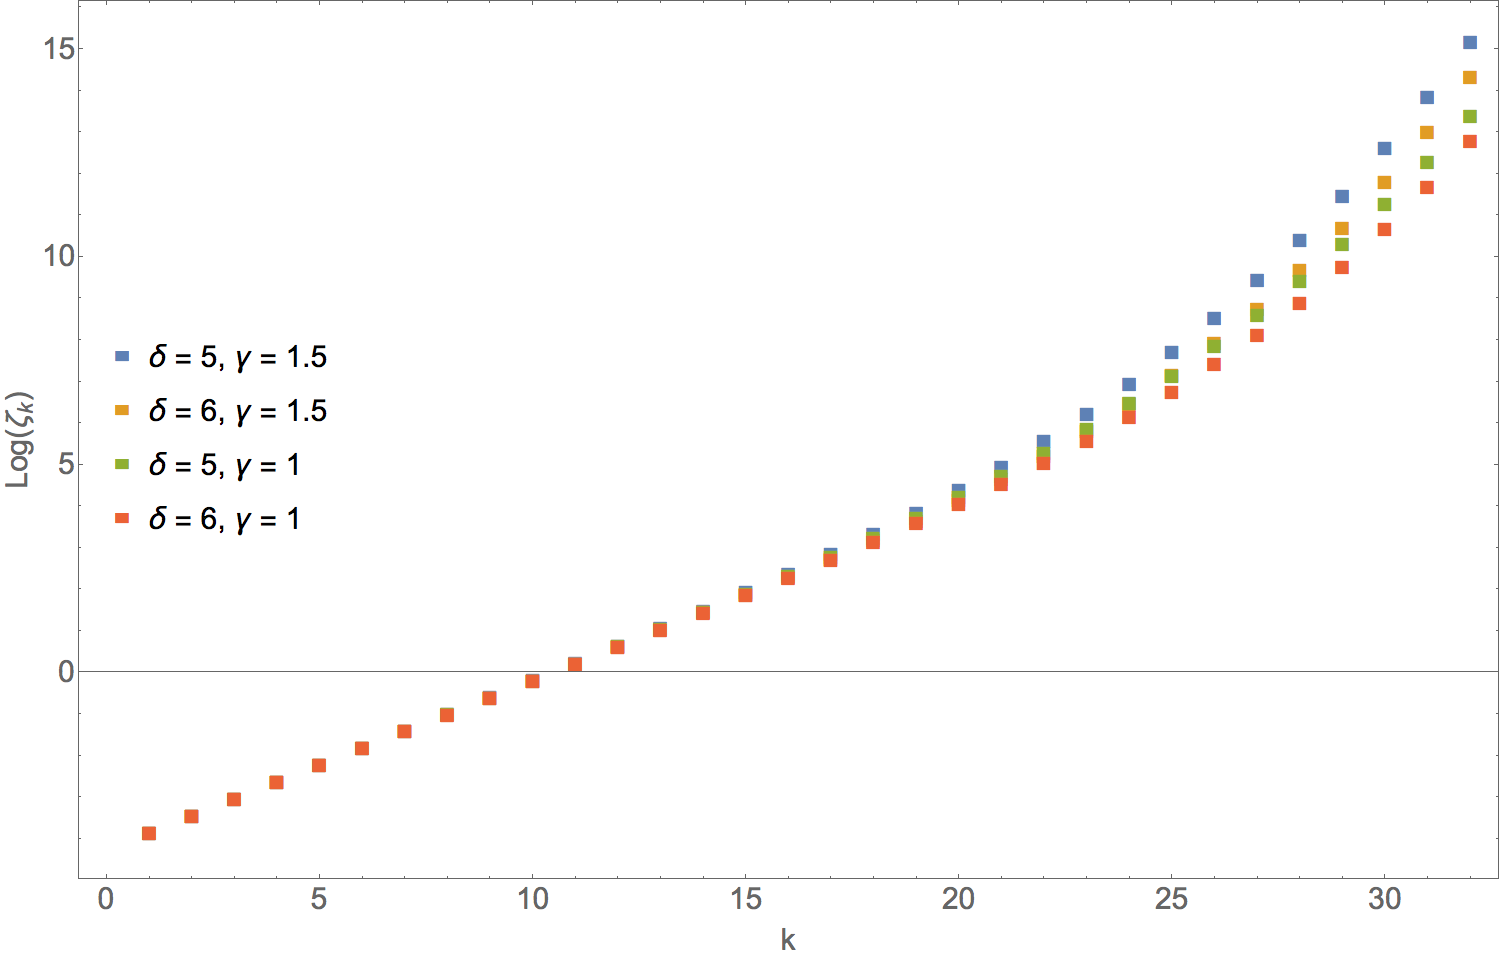
\includegraphics[width=1\textwidth]{Figures/deltagamm.png}
\caption[Changes in $\zeta$ as the values of $\delta$ and $\gamma$ are changed.]
{Changes in $\zeta$ as the values of $\delta$ and $\gamma$ are changed. The value of $n$ was 36, $\alpha$ was 0.02, and $\beta$ was 1.5}
\label{fig:deltagamm}
\end{figure}

It should be mentioned that each symmetry does not need to use the entire set of $\zeta$s that we optimize. Indeed, the most diffuse orbitals in the valence shells often don't use the most contracted functions at all, and conversely the most contracted orbitals in the core don't make much use of the most diffuse functions. Therefore, it is better to think of the set of $\zeta$s as pool, and that each symmetry is drawing a range of functions from that pool.  

\section{Methods}
\subsection{Basis set size optimization}
We decided to use a somewhat novel method of generating our basis sets. We begin by choosing an arbitrarily large basis set size, such as \mbox{s$(1:40)$p$(1:40)$d$(1:40)$f$(1:40)$} (here $i(\#:\#)$ refers to the starting and ending index of $\zeta$'s used for symmetry $i$). Next, we then find the optimal $\alpha$, $\beta$, $\delta$, and $\gamma$ WTBS parameters for this basis set. \notetodylan{This is done using NEWUOA\cite{Powell2006} which will find the values $\alpha$, $\beta$, $\delta$, and $\gamma$ that produce the lowest possible energy for a given basis set size.} Finally, we use the following steps to find the optimal basis set size.

\textit{Step 1.} Begin by finding the fewest number of f functions necessary. This can be done by generating input files that range in size from  \mbox{s$(1:40)$p$(1:40)$d$(1:40)$f$(1:1)$} to  \mbox{s$(1:40)$p$(1:40)$d$(1:40)$f$(1:40)$}.

\textit{Step 2.} Optimize the basis sets and select the smallest basis set that is still below some minimum accuracy threshold. We chose a relative error to numerical calculations of no greater than $5.0\times10^{-9}$ for non-relativistic sets and $5.0\times10^{-8}$ for relativistic sets where relative error is defined as $\frac{|(\text{optimized energy}) - (\text{numerical energy})|}{\text{numerical energy}}$. The size of this basis set is  \mbox{s$(1:40)$p$(1:40)$d$(1:40)$f$(1:x_{f})$}.

\textit{Step 3.} Replace the WTBS parameters with those from the newly optimized set and generate a list of input files that range in size from  \mbox{s$(1:40)$p$(1:40)$d$(1:x_{f})$f$(1:x_{f})$} to  \mbox{s$(1:40)$p$(1:40)$d$(1:40)$f$(1:x_{f})$}.

\textit{Step 4.} Optimize these new sets and select the smallest one that brings about an error that is still below the accuracy threshold. The size of this basis set is \\ \mbox{s$(1:40)$p$(1:40)$d$(1:x_{d})$f$(1:x_{f})$}.

\textit{Step 5.} Repeat steps 3 and 4 for the remaining symmetries. The size of the basis set at the end of this step will be of size  \mbox{s$(1:x_{s})$p$(1:x_{p})$d$(1:x_{d})$f$(1:x_{f})$}.

\textit{Step 6.} Replace the WTBS parameters with those from the newly optimized set and generate a list of input files that range in size from  \mbox{s$(1:x_{s})$p$(1:x_{p})$d$(1:x_{d})$f$(1:x_{f})$} to  \mbox{s$(1:x_{s})$p$(1:x_{p})$d$(1:x_{d})$f$(x_{f}:x_{f})$}.

\textit{Step 7.} Optimize and select from the basis sets. The new set will be of size  \\ \mbox{s$(1:x_{s})$p$(1:x_{p})$d$(1:x_{d})$f$(y_{f}:x_{f})$}.

\textit{Step 8.} Repeat steps 6 and 7 for the other symmetries except s. The final basis set will be of size  \mbox{s$(1:x_{s})$p$(y_{p}:x_{p})$d$(y_{d}:x_{d})$f$(y_{f}:x_{f})$}.

This procedure is perhaps a bit clunky, so let us work through an example using Ne. Ne has both s and p type orbitals, and so will our basis set. We might initially guess that no more than 26 functions per symmetry will enough to get the accuracy we want, so we start with a basis set of size s(1:26)p(1:26). We then optimize the $\alpha$, $\beta$, $\delta$, and $\gamma$ parameters for a basis set of this size. We make sure that the energy using a basis set of this size produces results that are accurate enough, and then we begin to reduce the size of the basis set for the p space. We carry over the WTBS parameters optimized in the last step, and generate input files corresponding to basis sets of size s(1:26)p(1:15) to s(1:26)p(1:26) (12 calculations in total) to determine the minimum number of tight functions we will need to accurately describe the p orbitals. After reoptimizing the WTBS parameters, we find that while s(1:26)p(1:15) is too small to be accurate enough, s(1:26)p(1:16) is still inside the threshold we want. So, we take the WTBS parameters from this calculation, and use them to generate new basis sets ranging in size from s(1:16)p(1:16) to s(1:26)p(1:16) (so we are trying to eliminate contracted functions from the s orbitals). Here we find that s(1:23)p(1:16) is the smallest basis set we can use. Now, we want to eliminate diffuse functions. Carrying over the WTBS parameter from the last acceptable basis set, we generate basis sets of size s(1:23)p(1:16) to s(1:23)p(5:16). We find that trying to remove any more functions makes the basis set unacceptable so we keep the s(1:23)p(1:16) basis set. We could try to remove diffuse functions from the s symmetry, but experience teaches that the s space needs all the functions to be accurate, so we don't bother.

This process has a major drawback in that it requires a lot of computer power to run efficiently. But this is not really a problem if access to large computer clusters is available. Additionally, considering that calculations for the chain 1-8 can be run in parallel for different atoms, this optimization process is trivially parallel. The advantages of this process are twofold: it finds a very small basis set that is still accurate and it is completely automatable. If there are no problems with individual calculations not converging, the output files never even need to be manually (and intellectually) examined! We generated non-relativistic basis sets for elements 2-86 using the rWTBS program\cite{WTBS, WTBS2, WTBS3, WTBS4, WTBS5, WTBS6} and relativistic basis sets for elements 55-86 using the cudaDFRATOM program which is outlined in detail in Chapter \ref{chp:cuda_dfratom}.

\subsection{Automating Optimization}
Automating the optimization process was quite simple. I did this by writing two scripts: BS\_sub\_auto\_rwtbs.sh and BS\_find\_best\_rwtbs.sh. The code for BS\_sub\_auto.sh is given here

\lstinputlisting[caption={BS\_sub\_auto\_rwtbs.sh},language=bash,framexrightmargin=15mm]{code_snippets/BS_sub_auto_rwtbs.sh}

The first few lines handle the arguments given to the script. The arguments are flags which tell the script what to do. The flags can be given in any order, so long as each flag is followed by the appropriate options. The default flag is a file ending in ``.inp" for the calculation that you would like to run. Optionally, this flag can be omitted, which will tell the script to run over all ``inp" files in the current directory. I will refer to the input file to be used as a seed. The flags ``-S", ``-P", ``-D", and ``-F" tell the script which set of orbitals we would like to remove functions from (``-S" means s orbitals, ``-P" means p orbitals, and so on). These flags \textit{\underline{must}} be followed by by two integers, with the first being smaller than the second. The first number is the minimum number for functions to cut, and the second is the maximum number to cut. By default, cutting begins with the most contracted function. For example, using ``-S 0 3" would take the seed file with a basis set of size s(1:20) and produce otherwise identical files with basis sets of size s(1:20), s(1:19), s(1:18), and s(1:17). If the number are negative, this can be used to add basis functions (``-S -1 0" on the same seed would produce basis sets of size s(1:21) and s(1:20)). Using the ``-B" (for bottom) flag changes the default behavior of cutting contracted functions, to cutting diffuse functions. So for example, using the flags ``-S 0 3 -B" on the seed would produce s(1:20), s(2:20), s(3:20), and s(4:20).

Once the flags have been parsed, the script makes a directory with the same name as the title of the seed, moves inside this directory, and generates the needed input files. It also creates a job submission script using the boilerplate function for each of new input files and submits them. Note that this part of the script will need to be changed depending on the cluster it is being used on. If more than one seed is used, then the script will do the same thing for each seed. After the jobs are completed, the user runs BS\_find\_best\_rwtbs.sh in the directory that contains all of the newly created directories. The code for BS\_find\_best\_rwtbs.sh is given below

\lstinputlisting[caption={BS\_find\_best\_rwtbs.sh},language=bash]{code_snippets/BS_find_best.sh}

This script takes in one argument, the relative error we are looking for in a calculation. It enters each of the subdirectories made by BS\_sub\_auto.sh and scans the output files for the relative error compared to numerical calculations. It finds the file with the smallest basis set that is still under the error threshold, and copies the input and output files for that calculation into a new directory called ``best". The user can then repeat this process for as many orbitals as they wish. There are also similar scripts for cudaDFRATOM which are given in Appendix \ref{app:cuda_dfratom_scripts}.

\section{Discussion}
\subsection{Optimized Non-Relativistic Basis Sets}
The optimized non-relativistic WTBS parameters and basis set sizes for elements 2-86 are shown in Table \ref{tab:BStab}. Relativistic WTBS parameters for elements 55-86 are shown in Table \ref{tab:BStab_rel}. Table \ref{tab:BStab_with_refs} gives the energies calculated with these basis sets compared to their literature values.

\begin{longtable}{l l r r r r r r r r}
\caption[Basis sets optimized using rWTBS]{Basis sets optimized using rWTBS. We did not have literature data for some elements. These elements are marked with a *. The size of the basis set for these elements was determined by using the size of the nearest elements.}\label{tab:BStab} \\
\toprule
	Element	&	Term		&	$\alpha$	&	$\beta$	&	$\delta$	&	$\gamma$	&	s	&	p	&	d	&	f	\\
			&	Symbol	&			&			&			&				&		&		&		&		\\
\midrule
\endfirsthead
\caption[]{(continued)}\\
\toprule
	Element	&	Term		&	$\alpha$	&	$\beta$	&	$\delta$	&	$\gamma$	&	s	&	p	&	d	&	f	\\
			&	Symbol	&			&			&			&				&		&		&		&		\\
\midrule
\endhead
02 He	& 	$^{1}S$  	&   	8.140$\times10^{-2}$   	&    	1.953    	&    	4.504    	&    	1.515    	&    	(1:18)    	\\
03 Li 	& 	$^{2}S$  	&   	1.596$\times10^{-2}$   	&    	1.933    	&    	5.701    	&    	1.573    	&    	(1:22)    	\\
04 Be 	& 	$^{1}S$  	&   	2.647$\times10^{-2}$   	&    	1.938    	&    	5.841    	&    	1.594    	&    	(1:22)    	\\	
05 B 		& 	$^{2}P$  	&   	3.238$\times10^{-2}$   	&    	1.948    	&    	5.573    	&    	1.523    	&    	(1:22)    	&    	(1:15)    	\\
06 C 	&  	$^{3}P$  	&   	4.613$\times10^{-2}$   	&    	1.941    	&    	4.717    	&    	1.317    	&    	(1:23)    	&    	(1:15)    	\\
07 N 	&  	$^{4}S$  	&   	5.976$\times10^{-2}$   	&    	1.923    	&    	5.183    	&    	1.442    	&    	(1:23)    	&    	(1:16)    	 \\
08 O 	&  	$^{3}P$  	&   	6.967$\times10^{-2}$   	&    	1.936    	&    	5.170    	&    	1.426    	&    	(1:23)    	&    	(1:16)    	\\
09 F 		&  	$^{2}P$  	&   	8.321$\times10^{-2}$   	&    	1.942    	&    	5.084    	&    	1.408    	&    	(1:23)    	&    	(1:16)    	\\
10 Ne 	&  	$^{1}S$  	&   	9.943$\times10^{-2}$   	&    	1.945    	&    	4.988    	&    	1.392    	&    	(1:23)    	&    	(1:16)    	\\
11 Na 	&  	$^{2}S$  	&   	1.696$\times10^{-2}$   	&    	1.950    	&    	6.056    	&    	1.469    	&    	(1:26)    	&    	(3:19)    	 \\
12 Mg 	&  	$^{1}S$  	&   	2.375$\times10^{-2}$   	&    	1.932    	&    	5.686    	&    	1.430    	&    	(1:26)    	&    	(3:19)    	\\
13 Al 	&  	$^{2}P$  	&   	2.239$\times10^{-2}$   	&    	1.898    	&    	5.555    	&    	1.413    	&    	(1:27)    	&    	(1:20)    	 \\
14 Si 	&  	$^{3}P$  	&   	3.352$\times10^{-2}$   	&    	1.921    	&    	5.419    	&    	1.410    	&    	(1:26)    	&    	(1:19)    	 \\
15 P 		&  	$^{4}S$  	&   	4.410$\times10^{-2}$   	&    	1.907    	&    	5.196    	&    	1.390    	&    	(1:26)    	&    	(1:19)    	    \\
16 S 		&  	$^{3}P$  	&   	5.004$\times10^{-2}$   	&    	1.896    	&    	4.962    	&    	1.362    	&    	(1:26)    	&    	(1:19)    	    \\
17 Cl 	&  	$^{2}P$  	&   	5.831$\times10^{-2}$   	&    	1.886    	&    	4.784    	&    	1.344    	&    	(1:26)    	&    	(1:19)    	    \\
18 Ar 	&  	$^{1}S$   	&   	6.834$\times10^{-2}$   	&    	1.878    	&    	4.654    	&    	1.331    	&    	(1:26)    	&    	(1:19)    	    \\
19 K 		&  	$^{2}S$   	&   	1.392$\times10^{-2}$   	&    	1.889    	&    	6.354    	&    	1.523    	&    	(1:28)    	&    	(3:22)    	    \\
20 Ca 	&  	$^{1}S$   	&   	1.837$\times10^{-2}$   	&    	1.874    	&    	6.109    	&    	1.504    	&    	(1:28)    	&    	(3:22)    	    \\
21 Sc 	&  	$^{2}D$   	&   	2.040$\times10^{-2}$   	&    	1.878    	&    	6.160    	&    	1.505    	&    	(1:28)    	&    	(3:22)    	&    	(2:16)   \\
22 Ti 	&  	$^{3}F$   	&   	2.218$\times10^{-2}$   	&    	1.886    	&    	6.247    	&    	1.508    	&    	(1:28)    	&    	(3:22)    	&    	(2:16)   \\
23 V 		&  	$^{4}F$   	&   	2.361$\times10^{-2}$   	&    	1.887    	&    	6.573    	&    	1.507    	&    	(1:29)    	&    	(3:23)    	&    	(2:16)   \\
24 Cr 	&  	$^{7}S$   	&   	2.345$\times10^{-2}$   	&    	1.865    	&    	5.348    	&    	1.407    	&    	(1:29)    	&    	(3:22)    	&    	(2:17)   \\
25 Mn 	&  	$^{6}S$   	&   	2.572$\times10^{-2}$   	&    	1.865    	&    	5.336    	&    	1.407    	&    	(1:29)    	&    	(3:22)    	&    	(2:17)   \\
26 Fe 	&  	$^{5}D$   	&   	2.621$\times10^{-2}$   	&    	1.869    	&    	5.301    	&    	1.395    	&    	(1:29)    	&    	(3:22)    	&    	(3:17)   \\
27 Co 	&  	$^{4}F$   	&   	2.643$\times10^{-2}$   	&    	1.871    	&    	5.905    	&    	1.413    	&    	(1:29)    	&    	(4:23)    	&    	(3:17)   \\
28 Ni 	&  	$^{3}F$   	&   	2.882$\times10^{-2}$   	&    	1.875    	&    	5.935    	&    	1.413    	&    	(1:29)    	&    	(3:23)    	&    	(3:17)   \\
29 Cu 	&  	$^{2}S$   	&   	2.283$\times10^{-2}$   	&    	1.857    	&    	5.485    	&    	1.413    	&    	(1:30)    	&    	(4:23)    	&    	(3:18)   \\
30 Zn 	&  	$^{1}S$   	&   	3.297$\times10^{-2}$   	&    	1.881    	&    	5.817    	&    	1.339    	&    	(1:30)    	&    	(3:24)    	&    	(2:17)   \\
31 Ga 	&  	$^{2}P$   	&   	2.742$\times10^{-2}$   	&    	1.863    	&    	5.703    	&    	1.462    	&    	(1:30)    	&    	(1:23)    	&    	(3:18)   \\
32 Ge 	&  	$^{3}P$   	&   	3.143$\times10^{-2}$   	&    	1.848    	&    	5.290    	&    	1.386    	&    	(1:30)    	&    	(1:23)    	&    	(4:18)   \\
33 As 	&  	$^{4}S$   	&   	4.728$\times10^{-2}$   	&    	1.869    	&    	5.325    	&    	1.340    	&    	(1:30)    	&    	(1:23)    	&    	(3:17)   \\
34 Se 	&	$^{3}P$   	&   	5.087$\times10^{-2}$   	&    	1.847    	&    	4.949    	&    	1.533    	&    	(1:30)    	&    	(1:22)    	&    	(3:18)   \\
35 Br 	&  	$^{2}P$   	&   	5.927$\times10^{-2}$   	&    	1.861    	&    	5.192    	&    	1.333    	&    	(1:30)    	&    	(1:23)    	&    	(3:17)   \\
36 Kr 	&  	$^{1}S$   	&   	6.804$\times10^{-2}$   	&    	1.859    	&    	5.510    	&    	1.370    	&    	(1:29)    	&    	(1:23)    	&    	(3:17)   \\
37 Rb 	&  	$^{2}S$   	&   	1.421$\times10^{-2}$   	&    	1.856    	&    	7.181    	&    	1.626    	&    	(1:30)    	&    	(3:25)    	&    	(6:21)   \\
38 Sr 	&  	$^{1}S$   	&   	1.808$\times10^{-2}$   	&    	1.846    	&    	6.674    	&    	1.553    	&    	(1:30)    	&    	(3:25)    	&    	(6:20)   \\
39 Y 		&  	$^{2}D$   	&   	1.997$\times10^{-2}$   	&    	1.841    	&    	6.569    	&    	1.543    	&    	(1:30)    	&    	(3:25)    	&    	(2:20)   \\
40 Zr 	&  	$^{5}F$   	&   	2.184$\times10^{-2}$   	&    	1.837    	&    	6.485    	&    	1.535    	&    	(1:30)    	&    	(3:25)    	&    	(2:20)   \\
41 Nb 	&  	$^{6}D$   	&   	2.340$\times10^{-2}$   	&    	1.835    	&    	6.434    	&    	1.530    	&    	(1:30)    	&    	(3:25)    	&    	(2:20)   \\
42 Mo 	&  	$^{7}S$   	&   	2.537$\times10^{-2}$   	&    	1.832    	&    	6.372    	&    	1.524    	&    	(1:30)    	&    	(3:25)    	&    	(2:20)   \\
43 Tc 	&  	$^{6}S$   	&   	2.597$\times10^{-2}$   	&    	1.836    	&    	6.453    	&    	1.534    	&    	(1:30)    	&    	(3:25)    	&    	(2:20)   \\
44 Ru 	&  	$^{5}F$   	&   	2.682$\times10^{-2}$   	&    	1.833    	&    	6.788    	&    	1.606    	&    	(1:30)    	&    	(3:25)    	&    	(2:21)   \\
45 Rh 	&  	$^{4}F$   	&   	2.751$\times10^{-2}$   	&    	1.835    	&    	6.883    	&    	1.620    	&    	(1:30)    	&    	(3:25)    	&    	(2:21)   \\
46 Pd 	&  	$^{1}S$   	&   	5.944$\times10^{-2}$   	&    	1.827    	&    	5.980    	&    	1.504    	&    	(1:29)    	&    	(2:24)    	&    	(1:19)   \\
47 Ag 	&  	$^{2}S$   	&   	2.438$\times10^{-2}$   	&    	1.800    	&    	5.521    	&    	1.423    	&    	(1:31)    	&    	(4:25)    	&    	(3:21)   \\
48 Cd 	&  	$^{1}S$   	&   	2.911$\times10^{-2}$   	&   	1.786   	&   	5.334   	&   	1.408   	&   	(1:31)   	&    	(4:25)    	&    	(3:21)   \\
49 In 	&  	$^{2}P$   	&   	2.714$\times10^{-2}$   	&    	1.799    	&    	5.540    	&    	1.431    	&    	(1:31)    	&    	(1:25)    	&    	(3:21)   \\
50 Sn 	&  	$^{3}P$   	&   	2.884$\times10^{-2}$   	&    	1.794    	&    	5.422    	&    	1.415    	&    	(1:31)    	&    	(1:25)    	&    	(4:21)   \\
51 Sb 	&  	$^{4}S$   	&   	4.481$\times10^{-2}$   	&    	1.815    	&    	6.567    	&    	1.605    	&    	(1:30)    	&   	(1:25)   	&    	(3:21)   \\
52 Te 	&  	$^{3}P$   	&   	4.846$\times10^{-2}$   	&    	1.817    	&    	6.247    	&    	1.528    	&    	(1:30)    	&    	(1:26)    	&    	(3:20)   \\
53 I 		&  	$^{2}P$   	&   	5.369$\times10^{-2}$   	&    	1.810    	&    	6.016    	&    	1.505    	&    	(1:30)    	&    	(1:25)    	&    	(3:20)   \\
54 Xe 	&  	$^{1}S$   	&   	5.981$\times10^{-2}$   	&    	1.802    	&    	5.862    	&    	1.490    	&    	(1:30)    	&    	(1:25)    	&    	(3:20)   \\
55 Cs 	&  	$^{2}S$   	&   	1.177$\times10^{-2}$   	&    	1.792    	&    	6.485    	&    	1.510    	&    	(1:33)    	&    	(4:28)    	&    	(5:23)   \\
56 Ba 	&  	$^{1}S$   	&   	1.560$\times10^{-2}$   	&    	1.770    	&    	6.152    	&    	1.518    	&    	(1:32)    	&    	(3:28)    	&    	(6:23)   \\
57 La 	&  	$^{2}D$   	&   	1.716$\times10^{-2}$   	&    	1.764    	&    	6.067    	&    	1.513    	&    	(1:32)    	&    	(3:28)    	&    	(2:23)     	&	(5:14)     	\\
58 Ce* 	&  	$^{3}H$   	&   	1.652$\times10^{-2}$   	&    	1.774    	&    	6.254    	&    	1.529    	&    	(1:32)    	&    	(3:28)    	&    	(2:23)     	&	(4:19)     	\\
59 Pr 	&  	$^{4}I$ 	&   	1.696$\times10^{-2}$   	&    	1.776    	&    	6.297    	&    	1.533    	&    	(1:32)    	&    	(3:28)    	&    	(6:23)     	& 	(4:19)     	\\
60 Nd 	&  	$^{5}I$ 	&   	1.737$\times10^{-2}$   	&    	1.778    	&    	6.563    	&    	1.579    	&    	(1:32)    	&    	(3:28)    	&    	(6:24)     	& 	(4:19)     	\\
61 Pm 	&  	$^{6}H$   	&   	1.784$\times10^{-2}$   	&    	1.780    	&    	6.615    	&    	1.585    	&    	(1:32)    	&    	(3:28)    	&    	(6:24)     	& 	(4:19)     	\\
62 Sm 	&  	$^{7}F$   	&   	1.857$\times10^{-2}$   	&    	1.778    	&    	5.842    	&    	1.464    	&    	(1:33)    	&    	(3:27)    	&    	(6:23)     	& 	(4:19)     	\\
63 Eu 	&  	$^{8}S$   	&   	1.876$\times10^{-2}$   	&    	1.784    	&    	6.718    	&    	1.596    	&    	(1:32)    	&    	(3:28)    	&    	(6:24)     	&  	(4:19)     	\\
64 Gd* 	&  	$^{7}F$   	&   	1.926$\times10^{-2}$   	&    	1.782    	&    	6.844    	&    	1.599    	&    	(1:33)    	&    	(3:28)    	&    	(6:24)     	&  	(4:19)     	\\
65 Tb* 	&  	$^{6}H$   	&   	1.971$\times10^{-2}$	&  	1.784	&   	6.898	&  	1.604	& 	(1:33) 	& 	(3:28) 	& 	(6:24)  	& 	(4:19)	\\   	   	   	
66 Dy 	&  	$^{5}I$ 	&   	2.020$\times10^{-2}$ 	& 	1.788 	& 	6.543 	& 	1.540 	& 	(1:33) 	& 	(3:28) 	& 	(6:23)  	& 	(4:19)	\\   	   	   	
67 Ho* 	&  	$^{4}I$ 	&   	2.064$\times10^{-2}$ 	&  	1.785	&    	7.090	&  	1.640	& 	(1:33) 	& 	(3:28) 	& 	(6:23)  	& 	(4:20)	\\   	   	  	
68 Er 	&  	$^{3}H$   	&   	2.106$\times10^{-2}$   	&   	1.792   	&   	7.029   	&   	1.638   	&   	(1:32)   	&   	(3:28)   	&   	(6:24)   	&   	(4:20)     	\\   	
69 Tm 	&  	$^{2}F$   	&   	2.152$\times10^{-2}$   	&   	1.794   	&   	7.075   	&   	1.643   	&   	(1:32)   	&   	(3:28)   	&   	(6:24)   	&   	(4:20)     	\\
70 Yb* 	&  	$^{1}S$   	&   	2.200$\times10^{-2}$   	&   	1.795   	&   	7.141   	&   	1.652   	&   	(1:32)   	&   	(3:28)   	&   	(2:24)   	&   	(4:20)     	\\   	
71 Lu 	&  	$^{2}D$   	&   	2.373$\times10^{-2}$   	&   	1.790   	&   	7.018   	&   	1.640   	&   	(1:32)   	&   	(3:28)   	&   	(2:24)   	&   	(4:20)     	\\   	
72 Hf 	& 	$^{3}F$   	&   	2.511$\times10^{-2}$   	&   	1.788   	&   	6.963   	&   	1.636   	&   	(1:32)   	&   	(3:28)   	&   	(2:24)   	&   	(5:20)     	\\   	
73 Ta 	& 	$^{4}F$   	&   	2.684$\times10^{-2}$   	&   	1.784   	&   	6.907   	&   	1.633   	&   	(1:32)   	&   	(2:28)   	&   	(2:24)   	&   	(5:20)     	\\   	
74 W 	& 	$^{5}D$   	&   	2.814$\times10^{-2}$   	&   	1.783   	&   	6.889   	&   	1.633   	&   	(1:32)   	&   	(3:28)   	&   	(2:24)   	&   	(5:20)     	\\   	
75 Re 	&	$^{6}S$   	&   	2.931$\times10^{-2}$   	&   	1.782   	&   	6.886   	&   	1.634   	&   	(1:32)   	&   	(3:28)   	&   	(2:24)   	&   	(5:20)     	\\   	
76 Os 	&  	$^{5}D$   	&   	3.075$\times10^{-2}$   	&   	1.781   	&   	6.896   	&   	1.637   	&   	(1:32)   	&   	(2:29)   	&   	(2:24)   	&   	(4:20)     	\\   	
77 Ir 		&  	$^{4}F$   	&   	3.195$\times10^{-2}$   	&   	1.780   	&   	6.867   	&   	1.635   	&   	(1:32)   	&   	(3:28)   	&   	(2:24)   	&   	(5:20)  	\\   	
78 Pt 	&  	$^{3}D$   	&   	3.173$\times10^{-2}$   	&   	1.785   	&   	7.020   	&   	1.654   	&   	(1:32)   	&   	(3:28)   	&   	(2:24)   	&   	(5:20)  	\\   	
79 Au 	&  	$^{2}S$   	&   	3.190$\times10^{-2}$   	&   	1.791   	&   	6.702   	&   	1.569   	&   	(1:33)   	&   	(4:28)   	&   	(2:23)   	&   	(5:19)  	\\   	
80 Hg 	&  	$^{1}S$   	&   	3.546$\times10^{-2}$   	&   	1.781   	&   	6.691   	&   	1.604   	&   	(1:32)   	&   	(3:28)   	&   	(2:23)   	&   	(5:20) 	\\   	
81 Tl 	&  	$^{2}P$   	&   	3.241$\times10^{-2}$   	&   	1.794   	&   	6.826   	&   	1.561   	&   	(1:34)   	&   	(1:29)   	&   	(3:23)   	&   	(6:20) 	\\   	
82 Pb 	&  	$^{3}P$   	&   	3.867$\times10^{-2}$   	&   	1.778   	&   	6.948   	&   	1.656   	&   	(1:32)   	&   	(1:28)   	&   	(3:25)   	&   	(6:21) 	\\   	
83 Bi 	&  	$^{4}S$   	&   	4.514$\times10^{-2}$   	&   	1.766   	&   	6.158   	&   	1.545   	&   	(1:32)   	&   	(1:27)   	&   	(2:24)   	&   	(6:19) 	\\   	
84 Po 	& 	$^{3}P$   	&   	4.783$\times10^{-2}$ 	& 	1.763 	& 	5.977 	& 	1.516 	& 	(1:32) 	& 	(1:27) 	& 	(3:23) 	& 	(6:19) 	\\   	
85 At 	& 	$^{2}P$ 	&   	5.210$\times10^{-2}$ 	& 	1.757 	& 	5.846 	& 	1.502 	& 	(1:32) 	& 	(1:27) 	& 	(3:23) 	& 	(6:19) 	\\
86 Rn 	& 	$^{1}S$ 	&   	5.716$\times10^{-2}$ 	& 	1.749 	& 	5.695 	& 	1.486 	& 	(1:32) 	& 	(1:27) 	& 	(3:23) 	& 	(6:19) 	\\
\bottomrule  	
\end{longtable}  	
  	
\begin{longtable}{l l r r r r r r r r}
\caption[Basis sets optimized using cudaDFRATOM]{Basis sets optimized using cudaDFRATOM}
\label{tab:BStab_rel} \\
\toprule
	Element	&	Electron		&	$\alpha$	&	$\beta$	&	$\delta$	&	$\gamma$	&	s	&	p	&	d	&	f	\\
			&	Configuration	&			&			&			&				&		&		&		&		\\
\midrule
\endfirsthead
\caption[]{(continued)}\\
\toprule
	Element	&	Electron		&	$\alpha$	&	$\beta$	&	$\delta$	&	$\gamma$	&	s	&	p	&	d	&	f	\\
			&	Configuration	&			&			&			&				&		&		&		&		\\
\midrule
\endhead
55 Cs		&	[Xe] 6s$^{1}$	&	1.824$\times10^{-2}$	&	1.921	&	6.085	&	1.062	&	(1:29)	&	 (3:28)	&	 (5:20)	\\
56 Ba		&	[Xe] 6s$^{2}$	&	2.033$\times10^{-2}$	&	1.904	&	5.473	&	1.161	&	(1:30)	&	 (3:28)	&	 (6:20)	\\
57 La		&	[Ba] 4f$^{1}$	&	1.540$\times10^{-2}$	&	1.871	&	5.166	&	2.036	&	(1:33)	&	 (4:28)	&	 (5:22)	&	 (4:16)\\
58 Ce		&	[Ba] 4f$^{2}$	&	1.838$\times10^{-2}$	&	1.857	&	4.969	&	1.450	&	(1:31)	&	 (3:28)	&	 (5:22)	&	 (4:16)\\
59 Pr		&	[Ba] 4f$^{3}$	&	1.945$\times10^{-2}$	&	1.857	&	4.947	&	1.438	&	(1:31)	&	 (3:28)	&	 (5:22)	&	 (4:16)\\
60 Nd		&	[Ba] 4f$^{4}$	&	2.043$\times10^{-2}$	&	1.859	&	4.928	&	1.422	&	(1:31)	&	 (3:28)	&	 (5:22)	&	 (4:16)\\
61 Pm		&	[Ba] 4f$^{5}$	&	2.142$\times10^{-2}$	&	1.860	&	4.906	&	1.405	&	(1:31)	&	 (2:28)	&	 (4:22)	&	 (4:16)\\
62 Sm		&	[Ba] 4f$^{6}$	&	2.414$\times10^{-2}$	&	1.856	&	4.854	&	1.379	&	(1:31)	&	 (3:28)	&	 (5:22)	&	 (3:16)\\
63 Eu		&	[Ba] 4f$^{7}$	&	1.993$\times10^{-2}$	&	1.877	&	5.099	&	1.020	&	(1:31)	&	 (4:29)	&	 (5:22)	&	 (4:16)\\
64 Gd		&	[Ba] 4f$^{8}$	&	2.063$\times10^{-2}$	&	1.880	&	5.064	&	0.996	&	(1:31)	&	 (4:29)	&	 (5:22)	&	 (4:16)\\
65 Td		&	[Ba] 4f$^{9}$	&	2.396$\times10^{-2}$	&	1.869	&	4.840	&	0.967	&	(1:31)	&	 (3:29)	&	 (5:22)	&	 (4:16)\\
66 Dy		&	[Ba] 4f$^{10}$	&	2.177$\times10^{-2}$	&	1.888	&	5.353	&	0.839	&	(1:30)	&	 (4:29)	&	 (5:22)	&	 (4:16)\\
67 Ho		&	[Ba] 4f$^{11}$	&	2.517$\times10^{-2}$	&	1.878	&	5.126	&	0.816	&	(1:30)	&	 (3:29)	&	 (5:22)	&	 (4:16)\\
68 Er		&	[Ba] 4f$^{12}$	&	2.811$\times10^{-2}$	&	1.875	&	5.145	&	1.045	&	(1:30)	&	 (3:29)	&	 (5:22)	&	 (3:16)\\
69 Tm		&	[Ba] 4f$^{13}$	&	2.628$\times10^{-2}$	&	1.887	&	5.480	&	0.886	&	(1:31)	&	 (3:30)	&	 (5:22)	&	 (4:16)\\
70 Yb		&	[Ba] 4f$^{14}$	&	2.918$\times10^{-2}$	&	1.883	&	5.490	&	0.873	&	(1:31)	&	 (3:30)	&	 (5:22)	&	 (3:16)\\
71 Lu		&	[Yb] 5d$^{1}$	&	3.424$\times10^{-2}$	&	1.873	&	5.124	&	1.353	&	(1:32)	&	 (2:29)	&	 (1:23)	&	 (3:16)\\
72 Hf		&	[Yb] 5d$^{2}$	&	3.982$\times10^{-2}$	&	1.900	&	6.117	&	1.473	&	(1:32)	&	 (2:29)	&	 (1:22)	&	 (4:16)\\
73 Ta		&	[Yb] 5d$^{3}$	&	4.271$\times10^{-2}$	&	1.899	&	6.126	&	1.450	&	(1:32)	&	 (3:29)	&	 (1:22)	&	 (4:16)\\
74 W			&	[Yb] 5d$^{4}$	&	4.564$\times10^{-2}$	&	1.901	&	5.936	&	1.351	&	(1:32)	&	 (3:29)	&	 (1:21)	&	 (4:16)\\
75 Re		&	[Yb] 5d$^{5}$	&	4.827$\times10^{-2}$	&	1.900	&	5.898	&	1.323	&	(1:32)	&	 (3:29)	&	 (1:21)	&	 (4:16)\\
76 Os		&	[Yb] 5d$^{6}$	&	5.081$\times10^{-2}$	&	1.899	&	5.873	&	1.296	&	(1:32)	&	 (3:29)	&	 (1:21)	&	 (4:16)\\
77 Ir		 	&	[Yb] 5d$^{7}$	&	5.333$\times10^{-2}$	&	1.898	&	5.846	&	1.274	&	(1:32)	&	 (3:29)	&	 (1:21)	&	 (4:16)\\
78 Pt		 	&	[Yb] 5d$^{8}$	&	5.391$\times10^{-2}$	&	1.892	&	6.058	&	1.365	&	(1:32)	&	 (3:29)	&	 (1:23)	&	 (5:16)\\
79 Au		&	[Yb] 5d$^{9}$	&	5.684$\times10^{-2}$	&	1.893	&	6.111	&	1.354	&	(1:32)	&	 (3:29)	&	 (1:23)	&	 (5:16)\\
80 Hg	 	&	[Yb] 5d$^{10}$	&	5.965$\times10^{-2}$	&	1.893	&	6.156	&	1.342	&	(1:32)	&	 (3:29)	&	 (1:23)	&	 (5:16)\\
81 Tl		 	&	[Hg] 6p$^{1}$	&	4.071$\times10^{-2}$	&	1.875	&	5.161	&	0.944	&	(1:30)	&	 (1:29)	&	 (1:22)	&	 (5:17)\\
82 Pb		&	[Hg] 6p$^{2}$	&	4.364$\times10^{-2}$	&	1.869	&	5.015	&	0.925	&	(1:30)	&	 (1:29)	&	 (3:22)	&	 (6:17)\\
83 Bi		 	&	[Hg] 6p$^{3}$	&	5.109$\times10^{-2}$	&	1.854	&	3.953	&	0.792	&	(1:33)	&	 (1:30)	&	 (2:21)	&	 (5:17)\\
84 Po		&	[Hg] 6p$^{4}$	&	5.439$\times10^{-2}$	&	1.849	&	4.666	&	0.890	&	(1:30)	&	 (1:29)	&	 (3:22)	&	 (6:17)\\
85 At		 	&	[Hg] 6p$^{5}$	&	6.177$\times10^{-2}$	&	1.892	&	10.223	&	1.500	&	(1:30)	&	 (1:31)	&	 (3:22)	&	 (6:16)\\
86 Rn	 	&	[Hg] 6p$^{6}$	&	6.671$\times10^{-2}$	&	1.831	&	3.906	&	0.867	&	(1:31)	&	 (1:29)	&	 (3:21)	&	 (6:17)\\
\bottomrule
\end{longtable}

\begin{longtable}{l r r r r}
\caption[Energies produced from basis sets in Tables \ref{tab:BStab} and \ref{tab:BStab_rel}]{Energies produced from basis sets in Tables \ref{tab:BStab} and \ref{tab:BStab_rel}. Relativistic basis sets are labeled with $^{r}$. All energies are in Hartree. Non-relativisic data comes from \cite{non_rel_lit_data}. Relativistic data comes from \cite{VISSCHER1997207}.}\label{tab:BStab_with_refs} \\
\toprule
	Element	  &	Calculated Energy		&	Literature Energy	&	Absolute Error	        &	Relative Error	        \\
			
\midrule
\endfirsthead
\caption[]{(continued)}\\
\toprule
	Element	  &	Calculated Energy   &	Literature Energy &   Absolute Error        &   Relative Error	      \\
\midrule
\endhead
02 He       &       -2.861        &     -2.861        &   $>1\times10^{-6}$     &   $3.6\times10^{-9}$    \\
03 Li       &       -7.432        &     -7.432        &   $>1\times10^{-6}$     &   $2.9\times10^{-9}$    \\
04 Be       &      -14.573        &    -14.573        &   $>1\times10^{-6}$     &   $3.2\times10^{-9}$    \\
05 B        &      -24.529        &    -24.529        &   $>1\times10^{-6}$     &   $4.8\times10^{-9}$    \\
06 C        &      -37.688        &    -37.688        &   $>1\times10^{-6}$     &   $4.1\times10^{-9}$    \\
07 N        &      -54.400        &    -54.400        &   $>1\times10^{-6}$     &   $2.8\times10^{-9}$    \\
08 O        &      -74.809        &    -74.809        &   $>1\times10^{-6}$     &   $3.4\times10^{-9}$    \\
09 F        &      -99.409        &    -99.409        &   $>1\times10^{-6}$     &   $4.0\times10^{-9}$    \\
10 Ne       &     -128.547        &   -128.547        &   $1\times10^{-6}$      &   $4.4\times10^{-9}$    \\
11 Na       &     -161.858        &   -161.858        &   $1\times10^{-6}$      &   $4.4\times10^{-9}$    \\
12 Mg       &     -199.614        &   -199.614        &   $1\times10^{-6}$      &   $3.9\times10^{-9}$    \\
13 Al       &     -241.876        &   -241.876        &   $1\times10^{-6}$      &   $2.8\times10^{-9}$    \\
14 Si       &     -288.854        &   -288.854        &   $1\times10^{-6}$      &   $4.6\times10^{-9}$    \\
15 P        &     -340.718        &   -340.718        &   $1\times10^{-6}$      &   $4.3\times10^{-9}$    \\
16 S        &     -397.504        &   -397.504        &   $2\times10^{-6}$      &   $4.5\times10^{-9}$    \\
17 Cl       &     -459.482        &   -459.482        &   $2\times10^{-6}$      &   $4.6\times10^{-9}$    \\
18 Ar       &     -526.817        &   -526.817        &   $2\times10^{-6}$      &   $4.5\times10^{-9}$    \\
19 K        &     -599.164        &   -599.164        &   $3\times10^{-6}$      &   $4.6\times10^{-9}$    \\
20 Ca       &     -676.758        &   -676.758        &   $3\times10^{-6}$      &   $3.8\times10^{-9}$    \\
21 Sc       &     -759.735        &   -759.735        &   $3\times10^{-6}$      &   $4.3\times10^{-9}$    \\
22 Ti       &     -848.405        &   -848.405        &   $4\times10^{-6}$      &   $4.9\times10^{-9}$    \\
23 V        &     -942.884        &   -942.884        &   $4\times10^{-6}$      &   $4.4\times10^{-9}$    \\
24 Cr       &    -1043.356        &  -1043.356        &   $4\times10^{-6}$      &   $4.1\times10^{-9}$    \\
25 Mn       &    -1149.866        &  -1149.866        &   $6\times10^{-6}$      &   $4.8\times10^{-9}$    \\
26 Fe       &    -1262.443        &  -1262.443        &   $6\times10^{-6}$      &   $4.5\times10^{-9}$    \\
27 Co       &    -1381.414        &  -1381.414        &   $6\times10^{-6}$      &   $4.6\times10^{-9}$    \\
28 Ni       &    -1506.870        &  -1506.870        &   $7\times10^{-6}$      &   $4.8\times10^{-9}$    \\
29 Cu       &    -1638.963        &  -1638.963        &   $6\times10^{-6}$      &   $3.4\times10^{-9}$    \\
30 Zn       &    -1777.848        &  -1777.848        &   $9\times10^{-6}$      &   $4.8\times10^{-9}$    \\
31 Ga       &    -1923.261        &  -1923.261        &   $9\times10^{-6}$      &   $4.5\times10^{-9}$    \\
32 Ge       &    -2075.359        &  -2075.359        &   $7\times10^{-6}$      &   $3.3\times10^{-9}$    \\
33 As       &    -2234.238        &  -2234.238        &   $1\times10^{-5}$      &   $4.8\times10^{-9}$    \\
34 Se       &    -2399.867        &  -2399.867        &   $1\times10^{-5}$      &   $4.4\times10^{-9}$    \\
35 Br       &    -2572.441        &  -2572.441        &   $1\times10^{-5}$      &   $4.8\times10^{-9}$    \\
36 Kr       &    -2752.054        &  -2752.054        &   $1\times10^{-5}$      &   $4.7\times10^{-9}$    \\
37 Rb       &    -2938.357        &  -2938.357        &   $1\times10^{-5}$      &   $4.7\times10^{-9}$    \\
38 Sr       &    -3131.545        &  -3131.545        &   $1\times10^{-5}$      &   $4.4\times10^{-9}$    \\
39 Y        &    -3331.684        &  -3331.684        &   $1\times10^{-5}$      &   $4.4\times10^{-9}$    \\
40 Zr       &    -3538.995        &  -3538.995        &   $1\times10^{-5}$      &   $4.4\times10^{-9}$    \\
41 Nb       &    -3753.597        &  -3753.597        &   $1\times10^{-5}$      &   $4.3\times10^{-9}$    \\
42 Mo       &    -3975.549        &  -3975.549        &   $1\times10^{-5}$      &   $4.5\times10^{-9}$    \\
43 Tc       &    -4204.788        &  -4204.788        &   $2\times10^{-5}$      &   $4.7\times10^{-9}$    \\
44 Ru       &    -4441.539        &  -4441.539        &   $2\times10^{-5}$      &   $4.5\times10^{-9}$    \\
45 Rh       &    -4685.881        &  -4685.881        &   $2\times10^{-5}$      &   $4.8\times10^{-9}$    \\
46 Pd       &    -4937.921        &  -4937.921        &   $2\times10^{-5}$      &   $4.8\times10^{-9}$    \\
47 Ag       &    -5197.698        &  -5197.698        &   $2\times10^{-5}$      &   $4.3\times10^{-9}$    \\
48 Cd       &    -5465.133        &  -5465.133        &   $2\times10^{-5}$      &   $4.2\times10^{-9}$    \\
49 In       &    -5740.169        &  -5740.169        &   $2\times10^{-5}$      &   $4.6\times10^{-9}$    \\
50 Sn       &    -6022.931        &  -6022.931        &   $2\times10^{-5}$      &   $3.9\times10^{-9}$    \\
51 Sb       &    -6313.485        &  -6313.485        &   $2\times10^{-5}$      &   $4.4\times10^{-9}$    \\
52 Te       &    -6611.784        &  -6611.784        &   $3\times10^{-5}$      &   $4.8\times10^{-9}$    \\
53 I        &    -6917.980        &  -6917.980        &   $3\times10^{-5}$      &   $4.6\times10^{-9}$    \\
54 Xe       &    -7232.138        &  -7232.138        &   $3\times10^{-5}$      &   $4.3\times10^{-9}$    \\
55 Cs       &    -7553.933        &  -7553.933        &   $2\times10^{-5}$      &   $3.6\times10^{-9}$    \\
56 Ba       &    -7883.543        &  -7883.543        &   $3\times10^{-5}$      &   $4.9\times10^{-9}$    \\
57 La       &    -8221.066        &  -8221.066        &   $4\times10^{-5}$      &   $4.8\times10^{-9}$    \\
58 Ce       &    -8566.919        &  -                &    -                    &    -                    \\
59 Pr       &    -8921.180        &  -8921.181        &   $4\times10^{-5}$      &   $4.9\times10^{-9}$   \\
60 Nd       &    -9283.882        &  -9283.882        &   $4\times10^{-5}$      &   $4.8\times10^{-9}$    \\
61 Pm       &    -9655.098        &  -9655.098        &   $4\times10^{-5}$      &   $4.7\times10^{-9}$    \\
62 Sm       &   -10034.952        & -10034.952        &   $4\times10^{-5}$      &   $4.4\times10^{-9}$    \\
63 Eu       &   -10423.543        & -10423.543        &   $4\times10^{-5}$      &   $4.7\times10^{-9}$    \\
64 Gd       &   -10820.617        & -                 &    -                    &    -                    \\
65 Tb       &   -11226.568        & -                 &    -                    &    -                    \\
66 Dy       &   -11641.452        & -11641.452        &   $5\times10^{-5}$      &   $4.4\times10^{-9}$    \\
67 Ho       &   -12065.289        & -                 &    -                    &    -                    \\
68 Er       &   -12498.152        & -12498.152        &   $6\times10^{-5}$      &   $4.8\times10^{-9}$    \\
69 Tm       &   -12940.174        & -12940.174        &   $6\times10^{-5}$      &   $4.8\times10^{-9}$    \\
70 Yb       &   -13391.456        & -                 &    -                    &    -                    \\
71 Lu       &   -13851.807        & -13851.808        &   $6\times10^{-5}$      &   $4.7\times10^{-9}$    \\
72 Hf       &   -14321.249        & -14321.249        &   $6\times10^{-5}$      &   $4.8\times10^{-9}$    \\
73 Ta       &   -14799.812        & -14799.812        &   $7\times10^{-5}$      &   $4.9\times10^{-9}$    \\
74 W        &   -15287.546        & -15287.546        &   $7\times10^{-5}$      &   $4.8\times10^{-9}$    \\
75 Re       &   -15784.533        & -15784.533        &   $7\times10^{-5}$      &   $4.9\times10^{-9}$    \\
76 Os       &   -16290.648        & -16290.648        &   $8\times10^{-5}$      &   $5.0\times10^{-9}$    \\
77 Ir       &   -16806.113        & -16806.113        &   $8\times10^{-5}$      &   $5.0\times10^{-9}$    \\
78 Pt       &   -17331.069        & -17331.069        &   $8\times10^{-5}$      &   $5.0\times10^{-9}$    \\
79 Au       &   -17865.399        & -17865.400        &   $8\times10^{-5}$      &   $4.9\times10^{-9}$    \\
80 Hg       &   -18408.991        & -18408.991        &   $9\times10^{-5}$      &   $5.0\times10^{-9}$    \\
81 Tl       &   -18961.824        & -18961.824        &   $8\times10^{-5}$      &   $4.6\times10^{-9}$    \\
82 Pb       &   -19524.008        & -19524.008        &   $9\times10^{-5}$      &   $4.9\times10^{-9}$    \\
83 Bi       &   -20095.586        & -20095.586        &   $1\times10^{-4}$      &   $5.0\times10^{-9}$    \\
84 Po       &   -20676.500        & -20676.500        &   $9\times10^{-5}$      &   $4.6\times10^{-9}$    \\
85 At       &   -21266.881        & -21266.881        &   $9\times10^{-5}$      &   $4.5\times10^{-9}$    \\
86 Rn       &   -21866.772        & -21866.772        &   $9\times10^{-5}$      &   $4.3\times10^{-9}$    \\
55 Cs$^{r}$ &    -7786.771        &  -7786.771        &   $3\times10^{-4}$      &   $4.6\times10^{-8}$    \\
56 Ba$^{r}$ &    -8135.644        &  -8135.645        &   $3\times10^{-4}$      &   $4.7\times10^{-8}$    \\
57 La$^{r}$ &    -8493.543        &  -8493.543        &   $4\times10^{-4}$      &   $4.8\times10^{-8}$    \\
58 Ce$^{r}$ &    -8860.997        &  -8860.997        &   $4\times10^{-4}$      &   $4.5\times10^{-8}$    \\
59 Pr$^{r}$ &    -9238.148        &  -9238.148        &   $4\times10^{-4}$      &   $4.6\times10^{-8}$    \\
60 Nd$^{r}$ &    -9625.131        &  -9625.131        &   $4\times10^{-4}$      &   $4.8\times10^{-8}$    \\
61 Pm$^{r}$ &   -10022.094        & -10022.095        &   $5\times10^{-4}$      &   $4.9\times10^{-8}$    \\
62 Sm$^{r}$ &   -10429.162        & -10429.163        &   $5\times10^{-4}$      &   $4.8\times10^{-8}$    \\
63 Eu$^{r}$ &   -10846.504        & -10846.505        &   $4\times10^{-4}$      &   $4.4\times10^{-8}$    \\
64 Gd$^{r}$ &   -11274.242        & -11274.242        &   $5\times10^{-4}$      &   $4.7\times10^{-8}$    \\
65 Td$^{r}$ &   -11712.544        & -11712.545        &   $5\times10^{-4}$      &   $4.3\times10^{-8}$    \\
66 Dy$^{r}$ &   -12161.545        & -12161.545        &   $6\times10^{-4}$      &   $4.9\times10^{-8}$    \\
67 Ho$^{r}$ &   -12621.412        & -12621.413        &   $5\times10^{-4}$      &   $4.6\times10^{-8}$    \\
68 Er$^{r}$ &   -13092.269        & -13092.270        &   $6\times10^{-4}$      &   $4.9\times10^{-8}$    \\
69 Tm$^{r}$ &   -13574.316        & -13574.317        &   $6\times10^{-4}$      &   $4.8\times10^{-8}$    \\
70 Yb$^{r}$ &   -14067.676        & -14067.677        &   $6\times10^{-4}$      &   $4.6\times10^{-8}$    \\
71 Lu$^{r}$ &   -14572.532        & -14572.533        &   $7\times10^{-4}$      &   $4.9\times10^{-8}$    \\
72 Hf$^{r}$ &   -15088.785        & -15088.786        &   $7\times10^{-4}$      &   $4.9\times10^{-8}$    \\
73 Ta$^{r}$ &   -15616.630        & -15616.630        &   $7\times10^{-4}$      &   $4.7\times10^{-8}$    \\
74 W$^{r}$  &   -16156.184        & -16156.185        &   $8\times10^{-4}$      &   $4.9\times10^{-8}$    \\
75 Re$^{r}$ &   -16707.619        & -16707.620        &   $8\times10^{-4}$      &   $4.9\times10^{-8}$    \\
76 Os$^{r}$ &   -17271.081        & -17271.082        &   $8\times10^{-4}$      &   $4.9\times10^{-8}$    \\
77 Ir$^{r}$ &   -17846.787        & -17846.788        &   $8\times10^{-4}$      &   $4.9\times10^{-8}$    \\
78 Pt$^{r}$ &   -18434.873        & -18434.874        &   $9\times10^{-4}$      &   $4.9\times10^{-8}$    \\
79 Au$^{r}$ &   -19035.525        & -19035.526        &   $9\times10^{-4}$      &   $4.9\times10^{-8}$    \\
80 Hg$^{r}$ &   -19648.895        & -19648.896        &   $9\times10^{-4}$      &   $4.9\times10^{-8}$    \\
81 Tl$^{r}$ &   -20274.849        & -20274.850        &   $9\times10^{-4}$      &   $4.8\times10^{-8}$    \\
82 Pb$^{r}$ &   -20913.713        & -20913.714        &   $9\times10^{-4}$      &   $4.7\times10^{-8}$    \\
83 Bi$^{r}$ &   -21565.705        & -21565.706        &   $1\times10^{-3}$      &   $4.9\times10^{-8}$    \\
84 Po$^{r}$ &   -22231.012        & -22231.013        &   $9\times10^{-4}$      &   $4.1\times10^{-8}$    \\
85 At$^{r}$ &   -22909.806        & -22909.807        &   $8\times10^{-4}$      &   $3.7\times10^{-8}$    \\
86 Rn$^{r}$ &   -23602.103        & -23602.104        &   $1\times10^{-3}$      &   $4.8\times10^{-8}$    \\
\bottomrule  	
\end{longtable}

In Table \ref{tab:dyall_comp}

\begin{table}
\caption[Comparison of basis sets produced by cudaDFRATOM and Dyall's triple-zeta basis sets.]{Comparison of basis sets produced by cudaDFRATOM and Dyall's triple-zeta basis sets. The basis sets for the 6s, 6p, and 5d elements are shown. The 4f elements were calculated with a different electron configuration, so they are omitted.} 
\label{tab:dyall_comp} \\
\begin{tabular}{l r r r r}
\toprule
  Element	  &	Calculated Energy$^{a}$ & Calculated Energy$^{b}$ & Total basis functions$^{a}$ & Total basis functions$^{b}$ 	      \\
\midrule
55 Cs &	-7786.771            &  -7786.771              & 113                         & 105  \\
56 Ba &	-8135.644            &  -8135.644              & 112                         & 104  \\
72 Hf &	-15088.785            & -15088.784              & 158                         & 129   \\
73 Ta &   -15616.630            & -15616.628              & 156                         & 129   \\
74 W &   -16156.184            & -16156.183              & 154                         & 129   \\
75 Re &   -16707.619            & -16707.617              & 154                         & 129   \\
76 Os &   -17271.081            & -17271.080              & 154                         & 129   \\
77 Ir &   -17846.787            & -17846.786              & 154                         & 129   \\
78 Pt	 &   -18434.873            & -18434.872              & 156                         & 129   \\
79 Au &   -19035.525            & -19035.526              & 156                         & 129   \\
80 Hg &   -19648.895            & -19648.893              & 156                         & 129   \\
81 Tl &   -20274.849            & -20274.850              & 158                         & 134   \\
82 Pb &   -20913.713            & -20913.714              & 152                         & 134   \\
83 Bi &   -21565.705            & -21565.706              & 156                         & 134   \\
84 Po &   -22231.012            & -22231.013              & 152                         & 134   \\
85 At &   -22909.806            & -22909.807              & 154                         & 134   \\
86 Rn &   -23602.103            & -23602.104              & 151                         & 134   \\
\bottomrule
\end{tabular}
  $^{a}$cudaDFRATOM basis sets	\\
  $^{b}$Dyalls basis sets
\end{table}

Figures \ref{fig:BS_non_rel_alpha}, \ref{fig:BS_non_rel_beta}, and \ref{fig:BS_non_rel_delt_gamm} show the trends of various non-relativistic parameters with respect to nuclear charge. In Figure  \ref{fig:BS_non_rel_alpha}, we can see that there is an interesting pattern where the exponent of the most diffuse function becomes larger as we move right across a row. It is also interesting to note that the rate at which the exponent increases changes when going from one block of that row to the next. The trend roughly follows what we expect from periodic trends of atomic size: atoms get larger by going left on the table. The trend of atoms getting larger when moving down the periodic table is mostly obeyed, however there are exceptions. For instance, the 4d elements have smaller values of $\alpha$ than the 5d elements.

In Figure \ref{fig:BS_non_rel_beta} shows that $\beta$ generally decreases as nuclear charge increases. As $\beta$ is involved in controlling the growth of the exponents, this indicates that the basis sets are getting more diffuse as the nuclear charge increases.

Finally \ref{fig:BS_non_rel_delt_gamm} shows the values of $\delta$ and $\gamma$ with respect to nuclear charge. There are no clear trends in these parameters, but they are shown for completeness.

\begin{figure}
\center
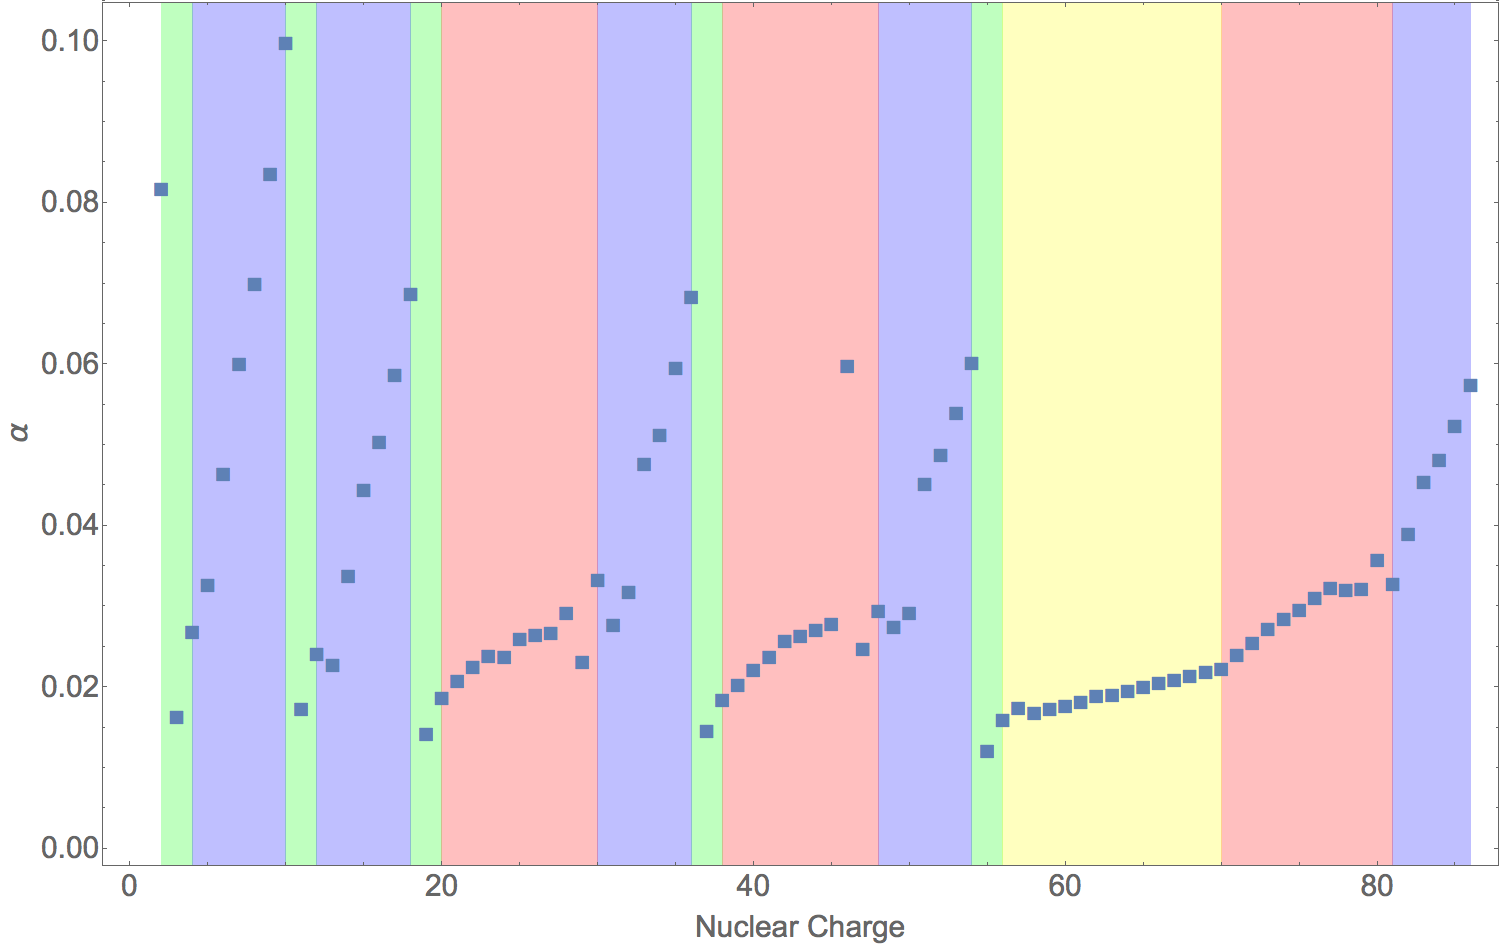
\includegraphics[width=1\textwidth]{Figures/BS_non_rel_alpha.png}
\caption[Scatter plot of the $\alpha$ parameter vs. nuclear charge.]
{Scatter plot of the $\alpha$ parameter vs. nuclear charge. Regions of the plot are shaded based on periodic table block regions. The s block is green, the p block is blue, the d block is red and the f block is yellow. There is a distinct pattern where the value of $\alpha$ increases along a row until a noble gas is reached. Also note how the rate of the increase changes at periodic table block boundaries.}
\label{fig:BS_non_rel_alpha}
\end{figure}

\begin{figure}
\center
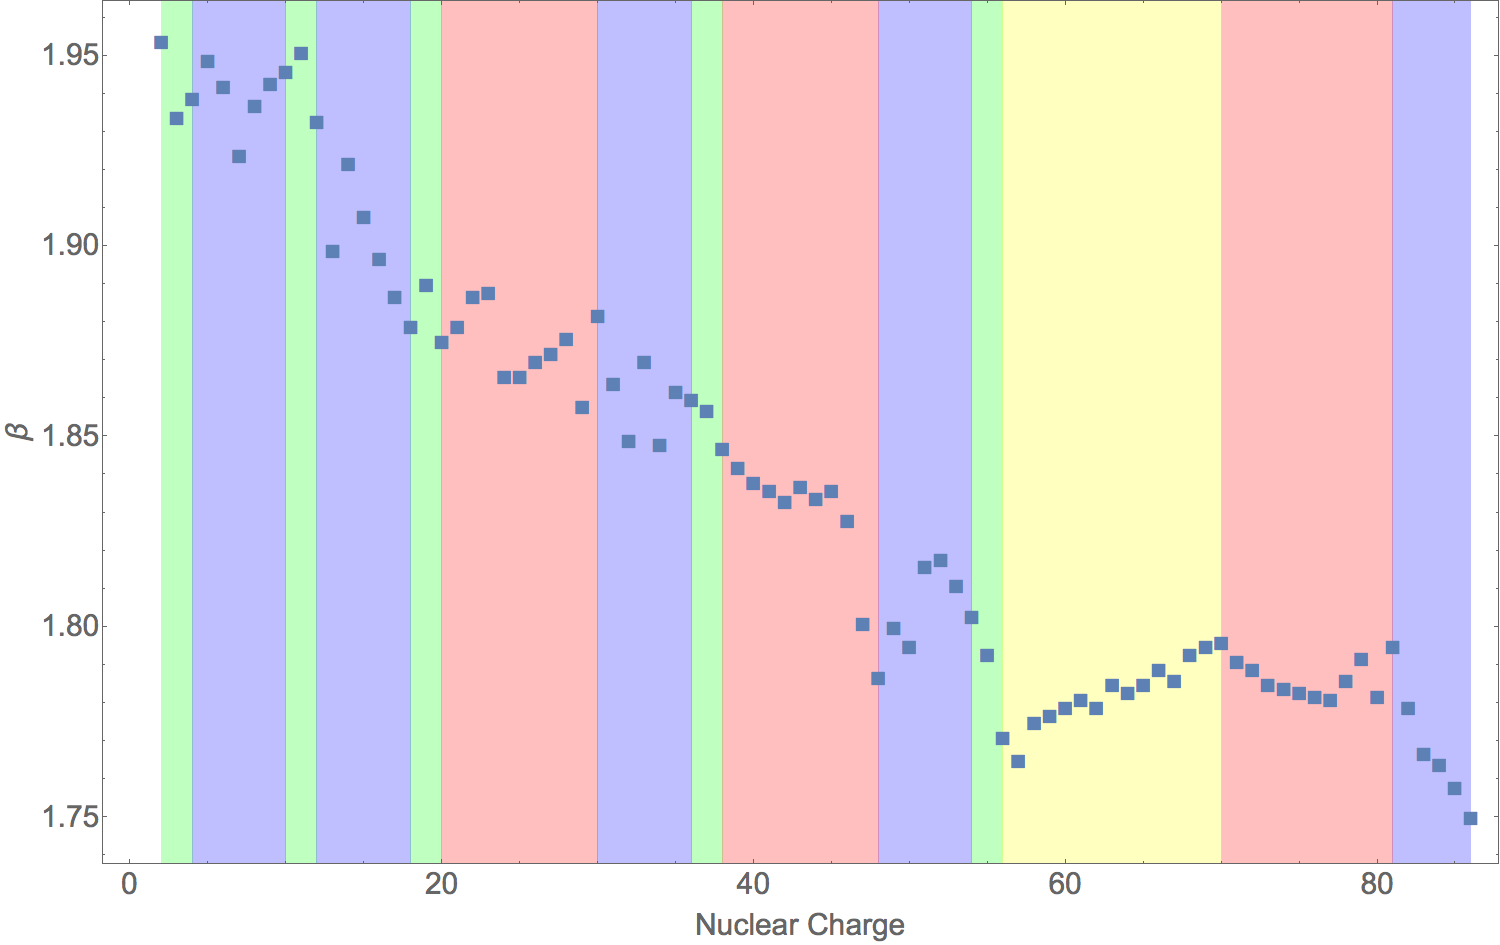
\includegraphics[width=1\textwidth]{Figures/BS_non_rel_beta.png}
\caption[Scatter plot of the $\beta$ parameter vs. nuclear charge.]
{Scatter plot of the $\beta$ parameter vs. nuclear charge. Regions of the plot are shaded based on periodic table block regions. The s block is green, the p block is blue, the d block is red and the f block is yellow. There is a general trend of the value of $\beta$ to decrease as the nuclear charge grows larger.}
\label{fig:BS_non_rel_beta}
\end{figure}

\begin{figure}
\centering
\begin{subfigure}[b]{0.49\textwidth}
	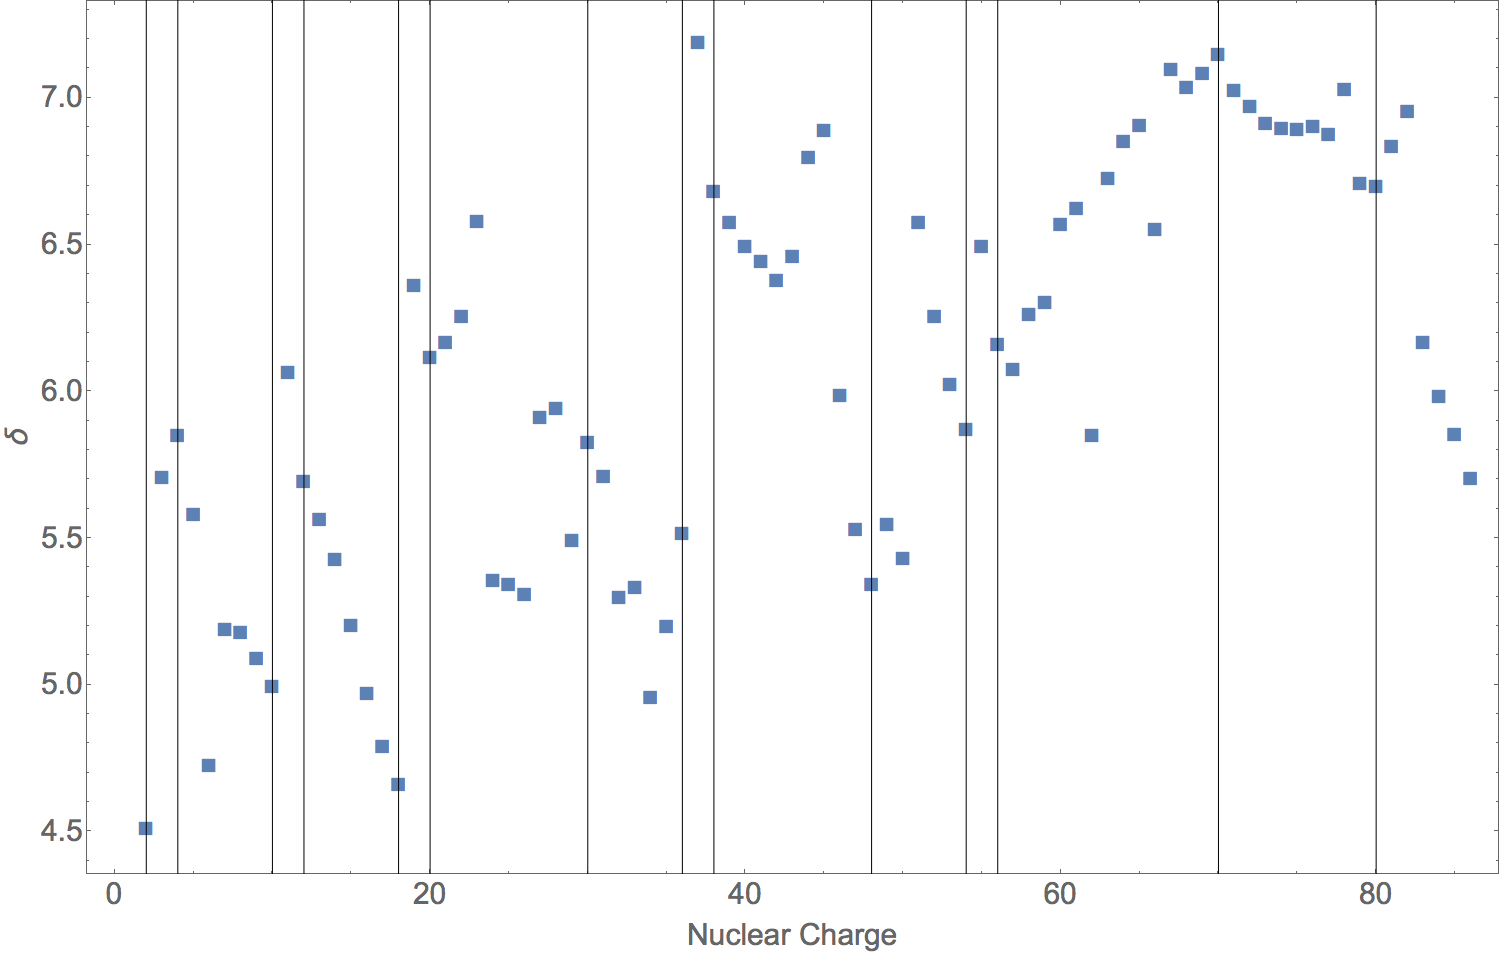
\includegraphics[width=\textwidth]{Figures/BS_non_rel_delta.png}
	\caption{$\delta$}
\end{subfigure}
\begin{subfigure}[b]{0.49\textwidth}
	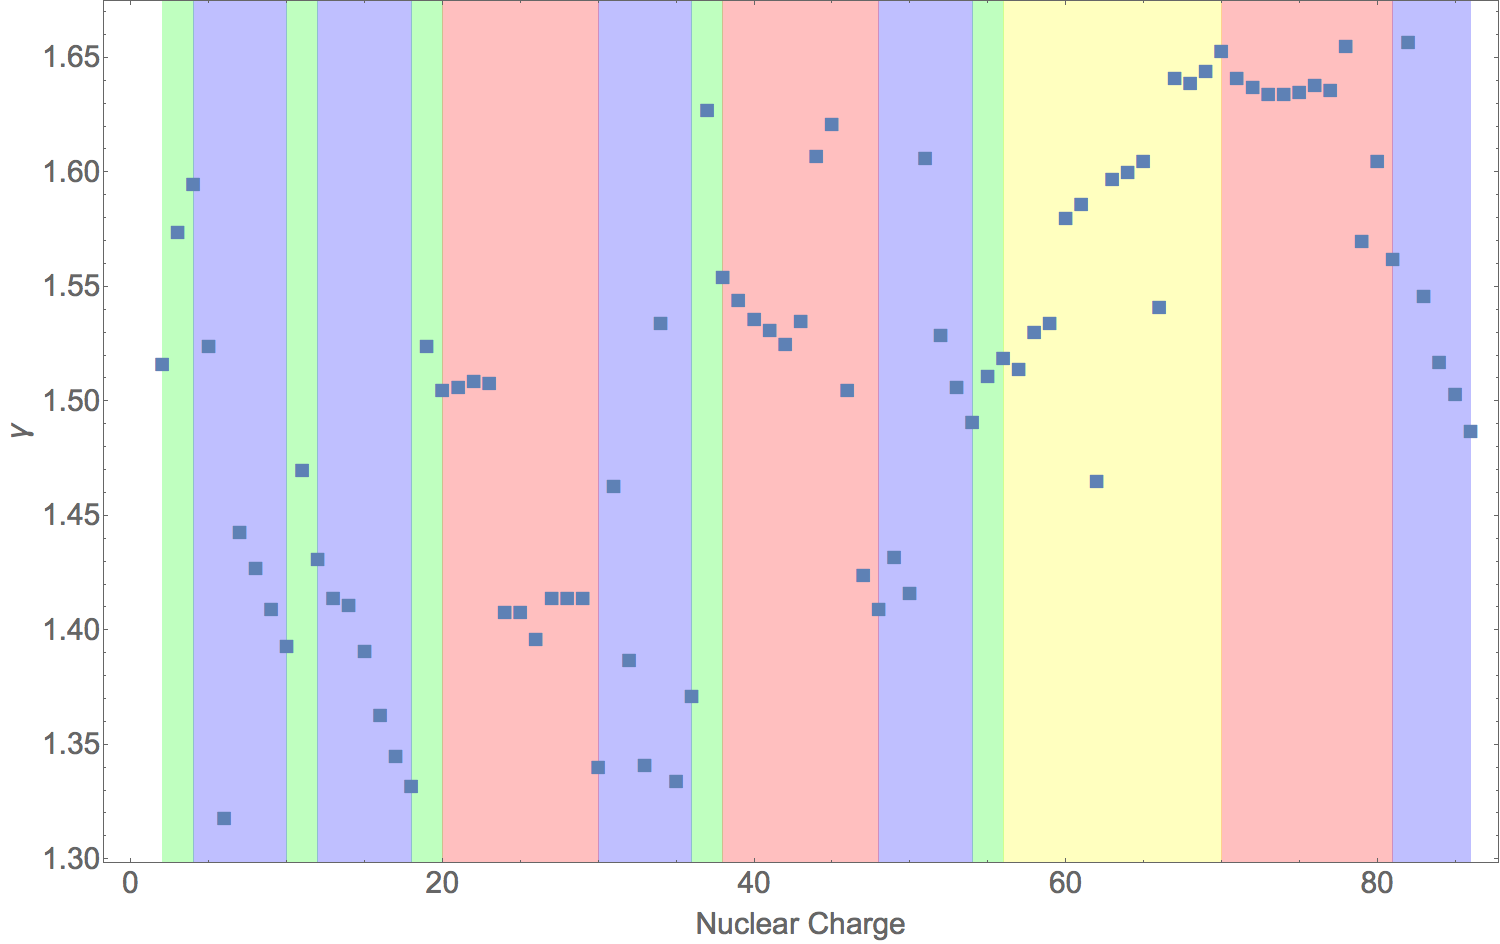
\includegraphics[width=\textwidth]{Figures/BS_non_rel_gamma.png}
	\caption{$\gamma$}
\end{subfigure}	
\caption[Scatter plots of the $\delta$ and $\gamma$ parameters.]{Scatter plots of the $\delta$ and $\gamma$ parameters. Regions of the plot are shaded based on periodic table block regions. The s block is green, the p block is blue, the d block is red and the f block is yellow. There are no clear trends with respect to the nuclear charge.}
\label{fig:BS_non_rel_delt_gamm}
\end{figure}

As for the relativistic basis sets, we can see from Figure \ref{fig:BS_rel_alpha} that the trend in $\alpha$ from the non-relativistic basis sets mostly holds, however there is a slight change in the trend starting at thallium. There is a substantial drop in the value of $\alpha$ when changing from the d to the p block in the relativistic basis sets which is not seen in the non-relativistic sets. We can also see that the change in $\alpha$ for the relativistic basis sets is much larger going through the d block than the change for the non-relativistic basis sets. As for the other WTBS parameters, the trends in the relativistic basis sets are mostly consistent with their non-relativistic counterparts. Figures for the remaining parameters are given in Figures \ref{fig:BS_rel_beta} and \ref{fig:BS_rel_delt_gamm}.

\begin{figure}
\center
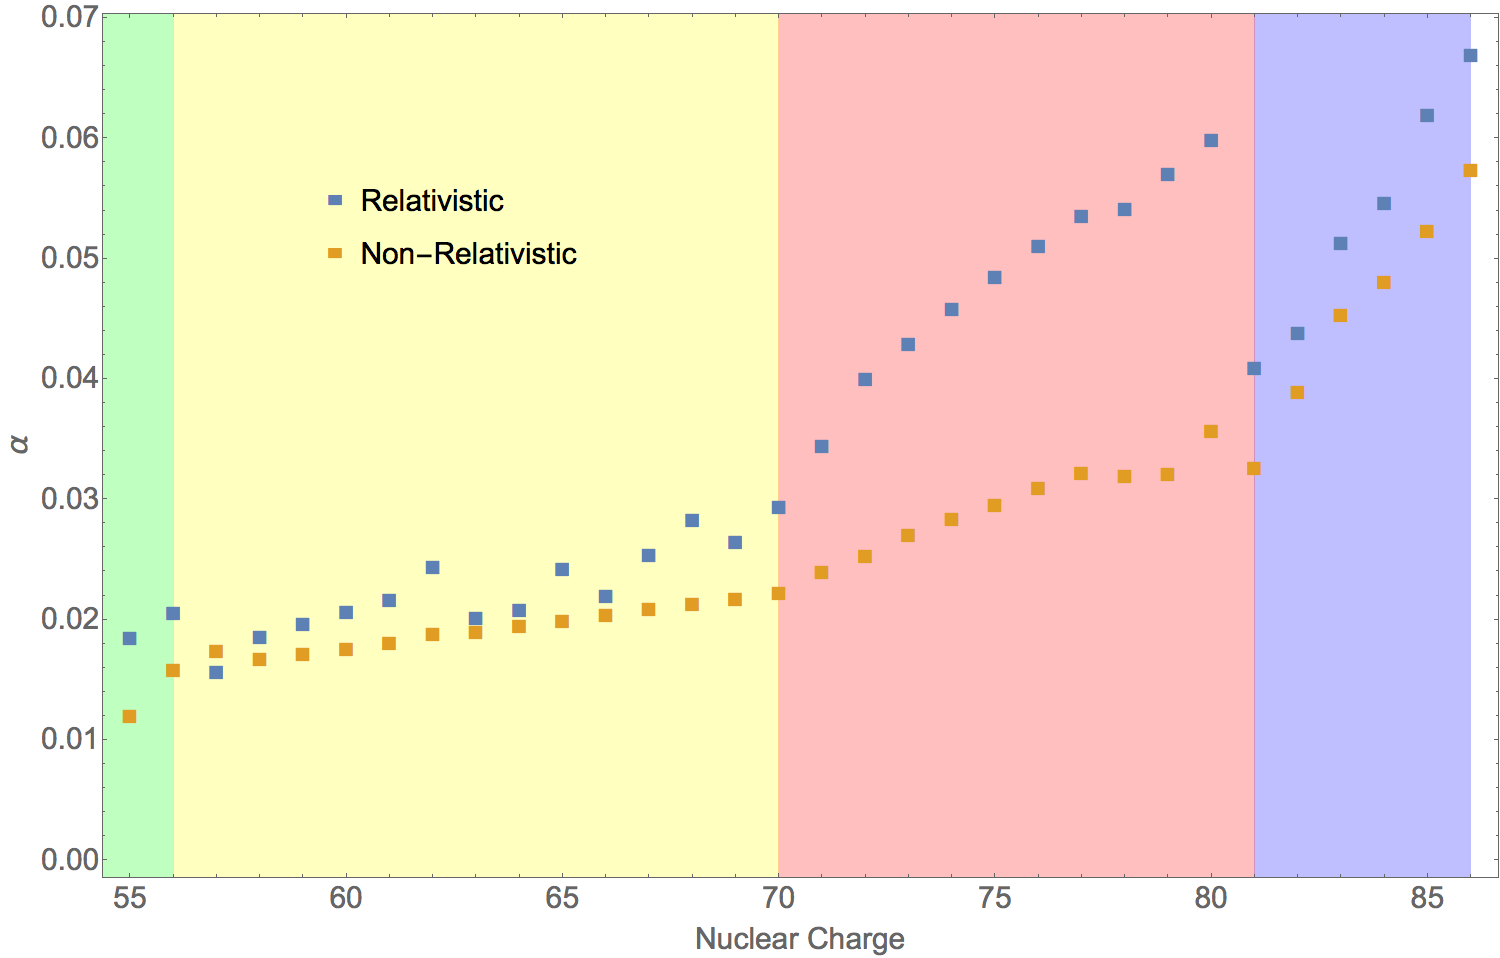
\includegraphics[width=1\textwidth]{Figures/BS_rel_alpha.png}
\caption[Scatter plot of the relativistic and non-relativistic $\alpha$ parameters vs. nuclear charge.]
{Scatter plot of the relativistic and non-relativistic $\alpha$ parameters vs. nuclear charge. Regions of the plot are shaded based on periodic table block regions. The s block is green, the p block is blue, the d block is red and the f block is yellow.}
\label{fig:BS_rel_alpha}
\end{figure}

\begin{figure}
\center
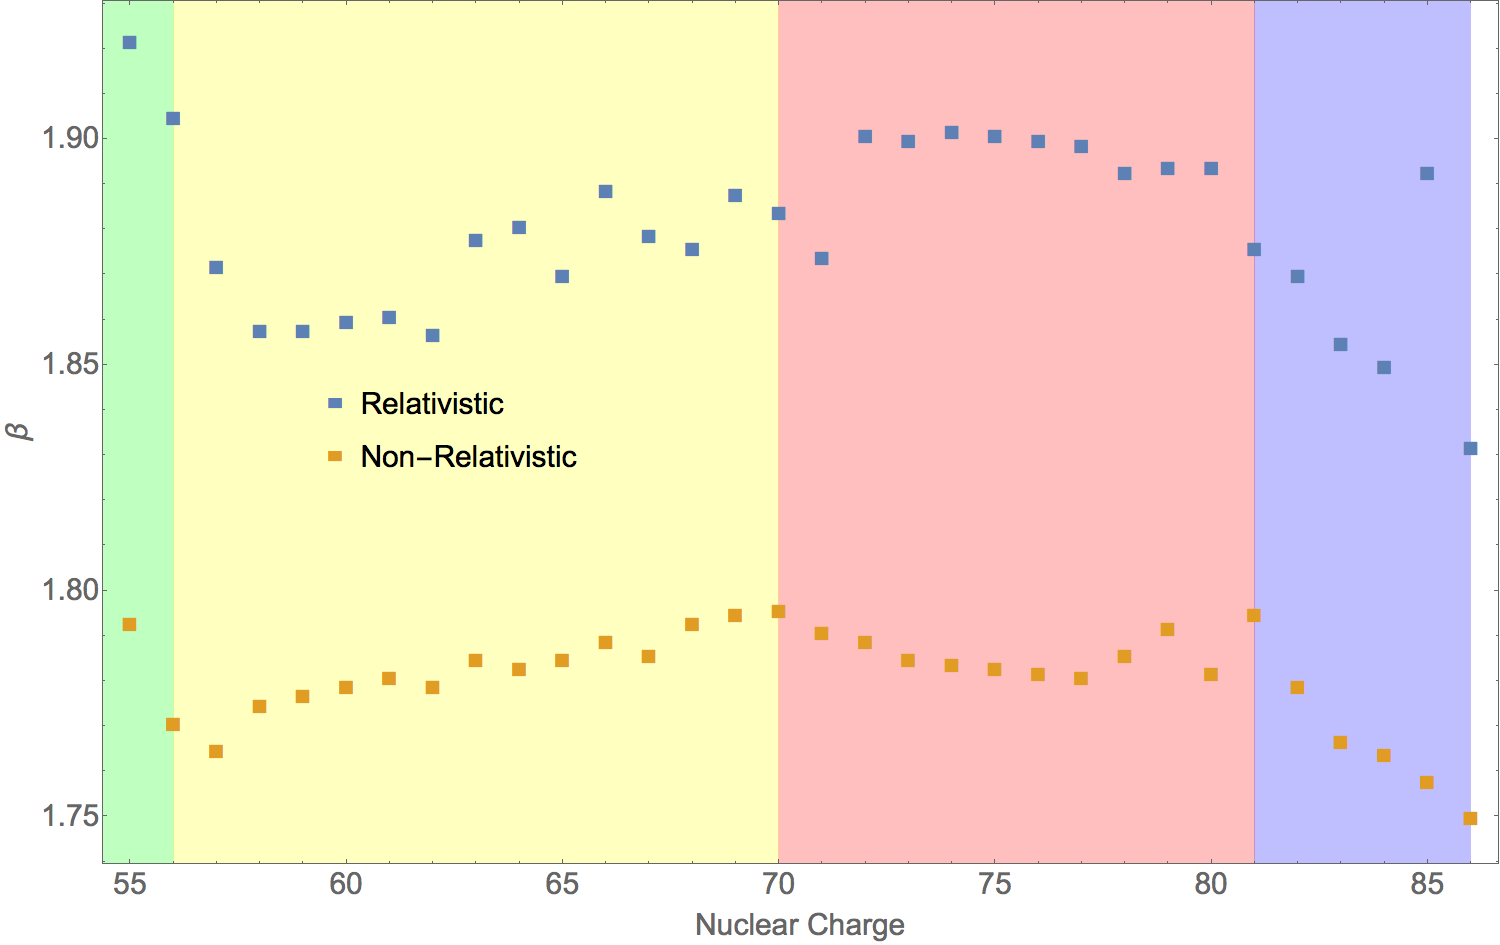
\includegraphics[width=1\textwidth]{Figures/BS_rel_beta.png}
\caption[Scatter plot of the relativistic and non-relativistic $\beta$ parameters vs. nuclear charge.]
{Scatter plot of the relativistic and non-relativistic $\beta$ parameters vs. nuclear charge. Regions of the plot are shaded based on periodic table block regions. The s block is green, the p block is blue, the d block is red and the f block is yellow.}
\label{fig:BS_rel_beta}
\end{figure}

\begin{figure}
\centering
\begin{subfigure}[b]{0.49\textwidth}
	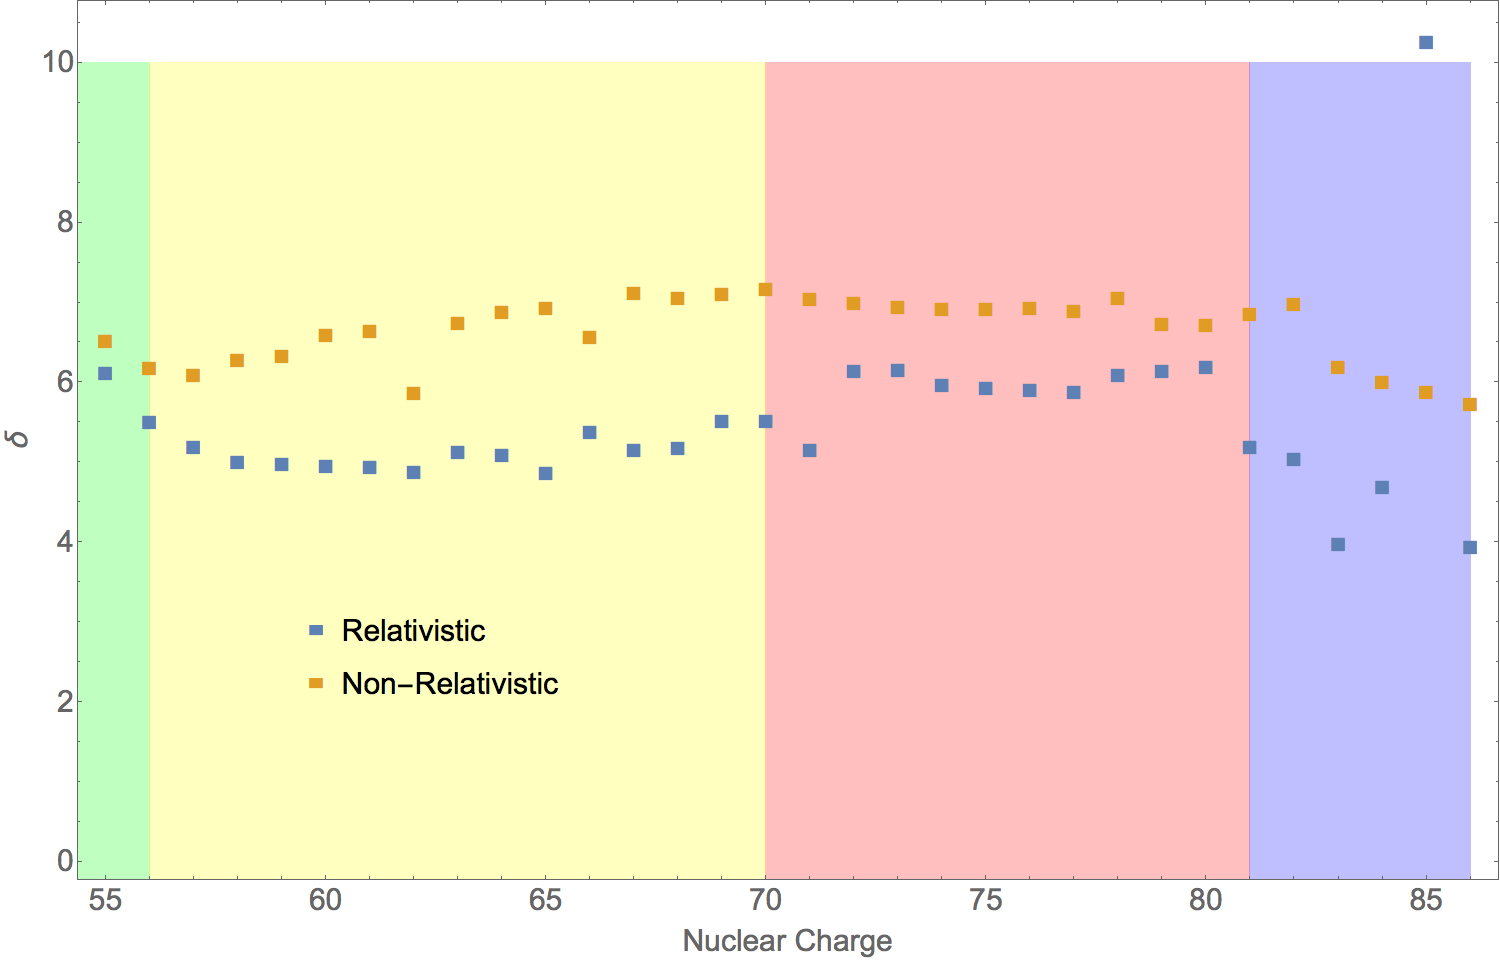
\includegraphics[width=\textwidth]{Figures/BS_rel_delta.png}
	\caption{$\delta$}
\end{subfigure}
\begin{subfigure}[b]{0.49\textwidth}
	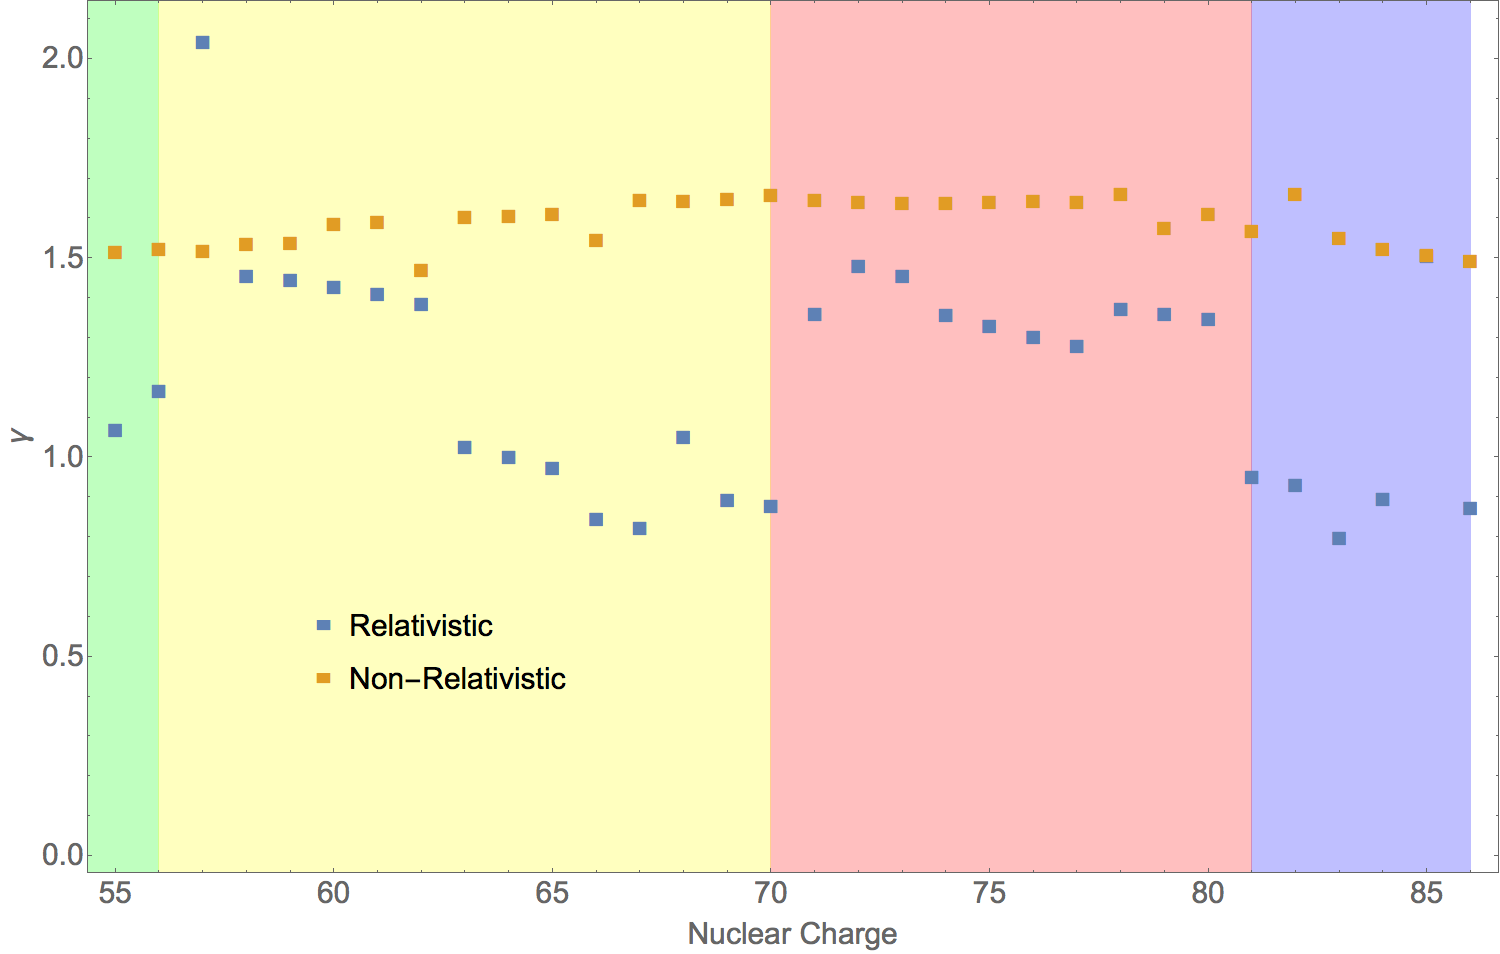
\includegraphics[width=\textwidth]{Figures/BS_rel_gamma.png}
	\caption{$\gamma$}
\end{subfigure}	
\caption[Scatter plot of the relativistic and non-relativistic $\delta$ and $\gamma$ parameters.]{Scatter plot of the relativistic and non-relativistic $\delta$ and $\gamma$ parameters. Regions of the plot are shaded based on periodic table block regions. The s block is green, the p block is blue, the d block is red and the f block is yellow.}
\label{fig:BS_rel_delt_gamm}
\end{figure}

